%% example.tex
%% Jeremy Singer
%% 16 Oct 12

\documentclass{mpaper}

\usepackage{mathtools}

\usepackage{tikz}
\usetikzlibrary{fit, arrows.meta, calc}

\usepackage{lipsum}

\usepackage{siunitx}
\usepackage[basic]{complexity}
\usepackage[super,negative]{nth}

\usepackage[linesnumbered,vlined,ruled,commentsnumbered]{algorithm2e}
\SetNlSty{}{}{}
\SetAlgoNlRelativeSize{-3}

\usepackage[labelfont=bf,textfont={bf,it}]{caption}
\usepackage{subcaption}
\captionsetup[subfigure]{justification=centering}
\usepackage{cleveref}

\usepackage{enumitem}
%\setlist{nosep}

\usepackage{booktabs}
\usepackage{microtype}

\usepackage[backend=bibtex,maxnames=3,maxbibnames=99,style=trad-abbrv]{biblatex}
\addbibresource{mprop.bib}

% Addendum formatting (thanks, http://tex.stackexchange.com/questions/339471/indented-addendums-using-biblatex-sourcemaps)
% Also remove doi, url since unnecessary
\DeclareFieldFormat{addendum}{}
%\DeclareFieldFormat{url}{}
%\DeclareFieldFormat{doi}{}
\DeclareFieldFormat*{url}{}
\DeclareFieldFormat[online]{url}{\mkbibacro{URL}\addcolon\space\url{#1}}
%\DeclareFieldFormat*{urldate}{}
%\DeclareFieldFormat[online]{urldate}{\mkbibparens{\bibstring{urlseen}\space#1}}

\usepackage{xpatch}

\xpatchbibmacro{name:andothers}{%
	\bibstring{andothers}%
}{%
	\bibstring[\emph]{andothers}%
}{}{}

\definecolor{graphc1}{RGB}{150,227,240}
\definecolor{graphc2}{RGB}{250,71,37}
\definecolor{graphc3}{RGB}{253,161,77}
\definecolor{graphc4}{RGB}{141,246,135}

% Official colours!

\definecolor{uofguniversityblue}{rgb}{0, 0.219608, 0.396078}

\definecolor{uofgheather}{rgb}{0.356863, 0.32549, 0.490196}
\definecolor{uofgaquamarine}{rgb}{0.603922, 0.72549, 0.678431}
\definecolor{uofgslate}{rgb}{0.309804, 0.34902, 0.380392}
\definecolor{uofgrose}{rgb}{0.823529, 0.470588, 0.709804}
\definecolor{uofgmocha}{rgb}{0.709804, 0.564706, 0.47451}

\definecolor{uofglawn}{rgb}{0.517647, 0.741176, 0}
\definecolor{uofgcobalt}{rgb}{0, 0.615686, 0.92549}
\definecolor{uofgturquoise}{rgb}{0, 0.709804, 0.819608}
\definecolor{uofgsunshine}{rgb}{1.0, 0.862745, 0.211765}
\definecolor{uofgpumpkin}{rgb}{1.0, 0.72549, 0.282353}
\definecolor{uofgthistle}{rgb}{0.584314, 0.070588, 0.447059}
\definecolor{uofgpillarbox}{rgb}{0.701961, 0.047059, 0}
\definecolor{uofglavendar}{rgb}{0.356863, 0.301961, 0.580392}

\definecolor{uofgsandstone}{rgb}{0.321569, 0.278431, 0.231373}
\definecolor{uofgforest}{rgb}{0, 0.317647, 0.2}
\definecolor{uofgburgundy}{rgb}{0.490196, 0.133333, 0.223529}
\definecolor{uofgrust}{rgb}{0.603922, 0.227451, 0.023529}

\newcommand{\lesspreceq}[1]{\prescript{}{#1}{\preceq}\ }

% Custom headings, sweet!
\newcommand{\subparagraph}{}
\usepackage[uppercase,tiny,noindentafter]{titlesec}
\titleformat{\subsection}{\normalfont\bfseries}{\thesubsection.}{1em}{}
\titleformat{\subsubsection}{\normalfont\bfseries}{\thesubsubsection.}{1em}{}
\titlelabel{\thetitle.\quad}
\titleformat{\paragraph}[runin]{\normalfont\normalsize\bfseries}{\theparagraph}{1em}{}

\begin{document}

\title{Graph Models and Maximum Common Subgraph for Character Analysis}
\author{Kyle A. Simpson}
\matricnum{2029567}

\maketitle
%====================================================
%====================================================
\begin{abstract}
%According to Simon Peyton Jones, an abstract should address
%four key questions. First, what is the problem that this
%paper tackles? Second, why is this an interesting problem?
%Third, what is the solution this paper proposes?
%Finally, why is the proposed solution a good one?
%Lorem ipsum dolor sit amet lorem ipsum dolor sit amet lorem ipsum dolor sit amet lorem ipsum dolor sit amet lorem ipsum dolor sit amet lorem ipsum dolor sit amet lorem ipsum dolor sit amet lorem ipsum dolor sit amet lorem ipsum dolor sit amet lorem ipsum dolor sit amet lorem ipsum dolor sit amet lorem ipsum dolor sit amet lorem ipsum dolor sit amet lorem ipsum dolor sit amet lorem ipsum dolor sit amet lorem ipsum dolor sit amet lorem ipsum dolor sit amet lorem ipsum dolor sit amet lorem ipsum dolor sit amet lorem ipsum dolor sit amet lorem ipsum dolor sit amet
\lipsum[1]

?? Write me
\end{abstract}
%====================================================
%====================================================

%====================================================
\section{Introduction}
\label{sec:introduction}
%====================================================

%?? Adapt proposal introduction
Research into computer vision tasks, such as image and object recognition, is currently dominated by the use of machine learning and vector-space models, while graph encodings are comparatively less well-explored.
%Neural networks and similar machine learning constructs learn features of the inputs and data they are given, which are later used to classify or identify patterns in images or generic datasets---and have become popular due to their versatility, effectiveness and accuracy across many problem domains.
Machine learning methods apply statistical inference from training data to teach classifiers how to recognise the desired elements or features from an image---and have become popular due to their versatility, effectiveness and accuracy across many problem domains.
Vector-space models, on the other hand, capture the area around high-contrast regions in images as salient features, or describe an image's contents in a dense and very low-level fashion.

In many cases it can be hard to reason about such models' robustness or sensitivity to different phenomena.
In a machine learning context, for instance, these are often a function of both the training data and the model itself.
The parameters learned by these models aren't structured in a way that allows humans to easily intuit what the model has learned or to comment on the system's correctness, and it can be difficult to discern \textit{why} a particular image might be misclassified.
Recent work into \emph{adversarial images} \cite{AdversarialML} has affirmed this, given that interference can lead to classifications contrary to image content.
%Outside of this, vector-space models can represent image interest points in a way that describes their neighbourhood (or indeed, the entirety of an image), and so are easier to understand; yet they lack any way to describe the relationships between these points or to capture an object's shape.

%?? Adversarial examples in ML \cite{AdversarialML}

Graph models, long-explored in discrete mathematics, provide a simpler way of visualising problems.
Systems are broken down into \emph{vertices} and \emph{edges} between vertex pairs---capturing the relationships between objects or key features within a scene.
For many domains, this is an intuitive and effective representation, encoding rich semantics in a very natural way which enjoys use in computational chemistry \cite{Graph-Molecules-2,Graph-Molecules-3,Graph-Molecules-1}, biology \cite{Graph-Biology-1}, and graph database analysis.
Furthermore, exact graph search and similarity metrics (e.g.\ the \emph{subgraph isomorphism} and \emph{maximum common subgraph} problems, respectively) are well-understood and an area of continual research in the field of algorithms.
%?? part of idea---need effective models to know that our similarity algorithms are a good fit?

The main aim of this paper is to explore the hypothesis that, after suitable transformation, image similarity corresponds to graph similarity according to these known metrics; \cref{fig:intro-sim} gives a rough illustration of the concept.
In particular, this work focuses on character analysis and recognition, considering both the performance of graph models within a domain alongside the usefulness of any chosen analytic techniques.
By investigating these questions, this paper contributes:
\begin{itemize}
	\item A demonstration of the shortcomings of existing image graph work for generic matching (\Cref{sec:image-weakness}), by attempting similarity computation on graphs built using common techniques from the literature. %given that this also requires an investigation into the effectiveness of known graph similarity techniques, this motivates the development of new models.
	This weakness motivates the development of new modelling strategies.
	\item ?? Detail as paper written
\end{itemize}

\begin{figure}
	\centering
	\resizebox{\columnwidth}{!}{
		\Large
		\begin{tikzpicture}
		\node[inner sep=5pt] (sagrada1) at (0,0)
		{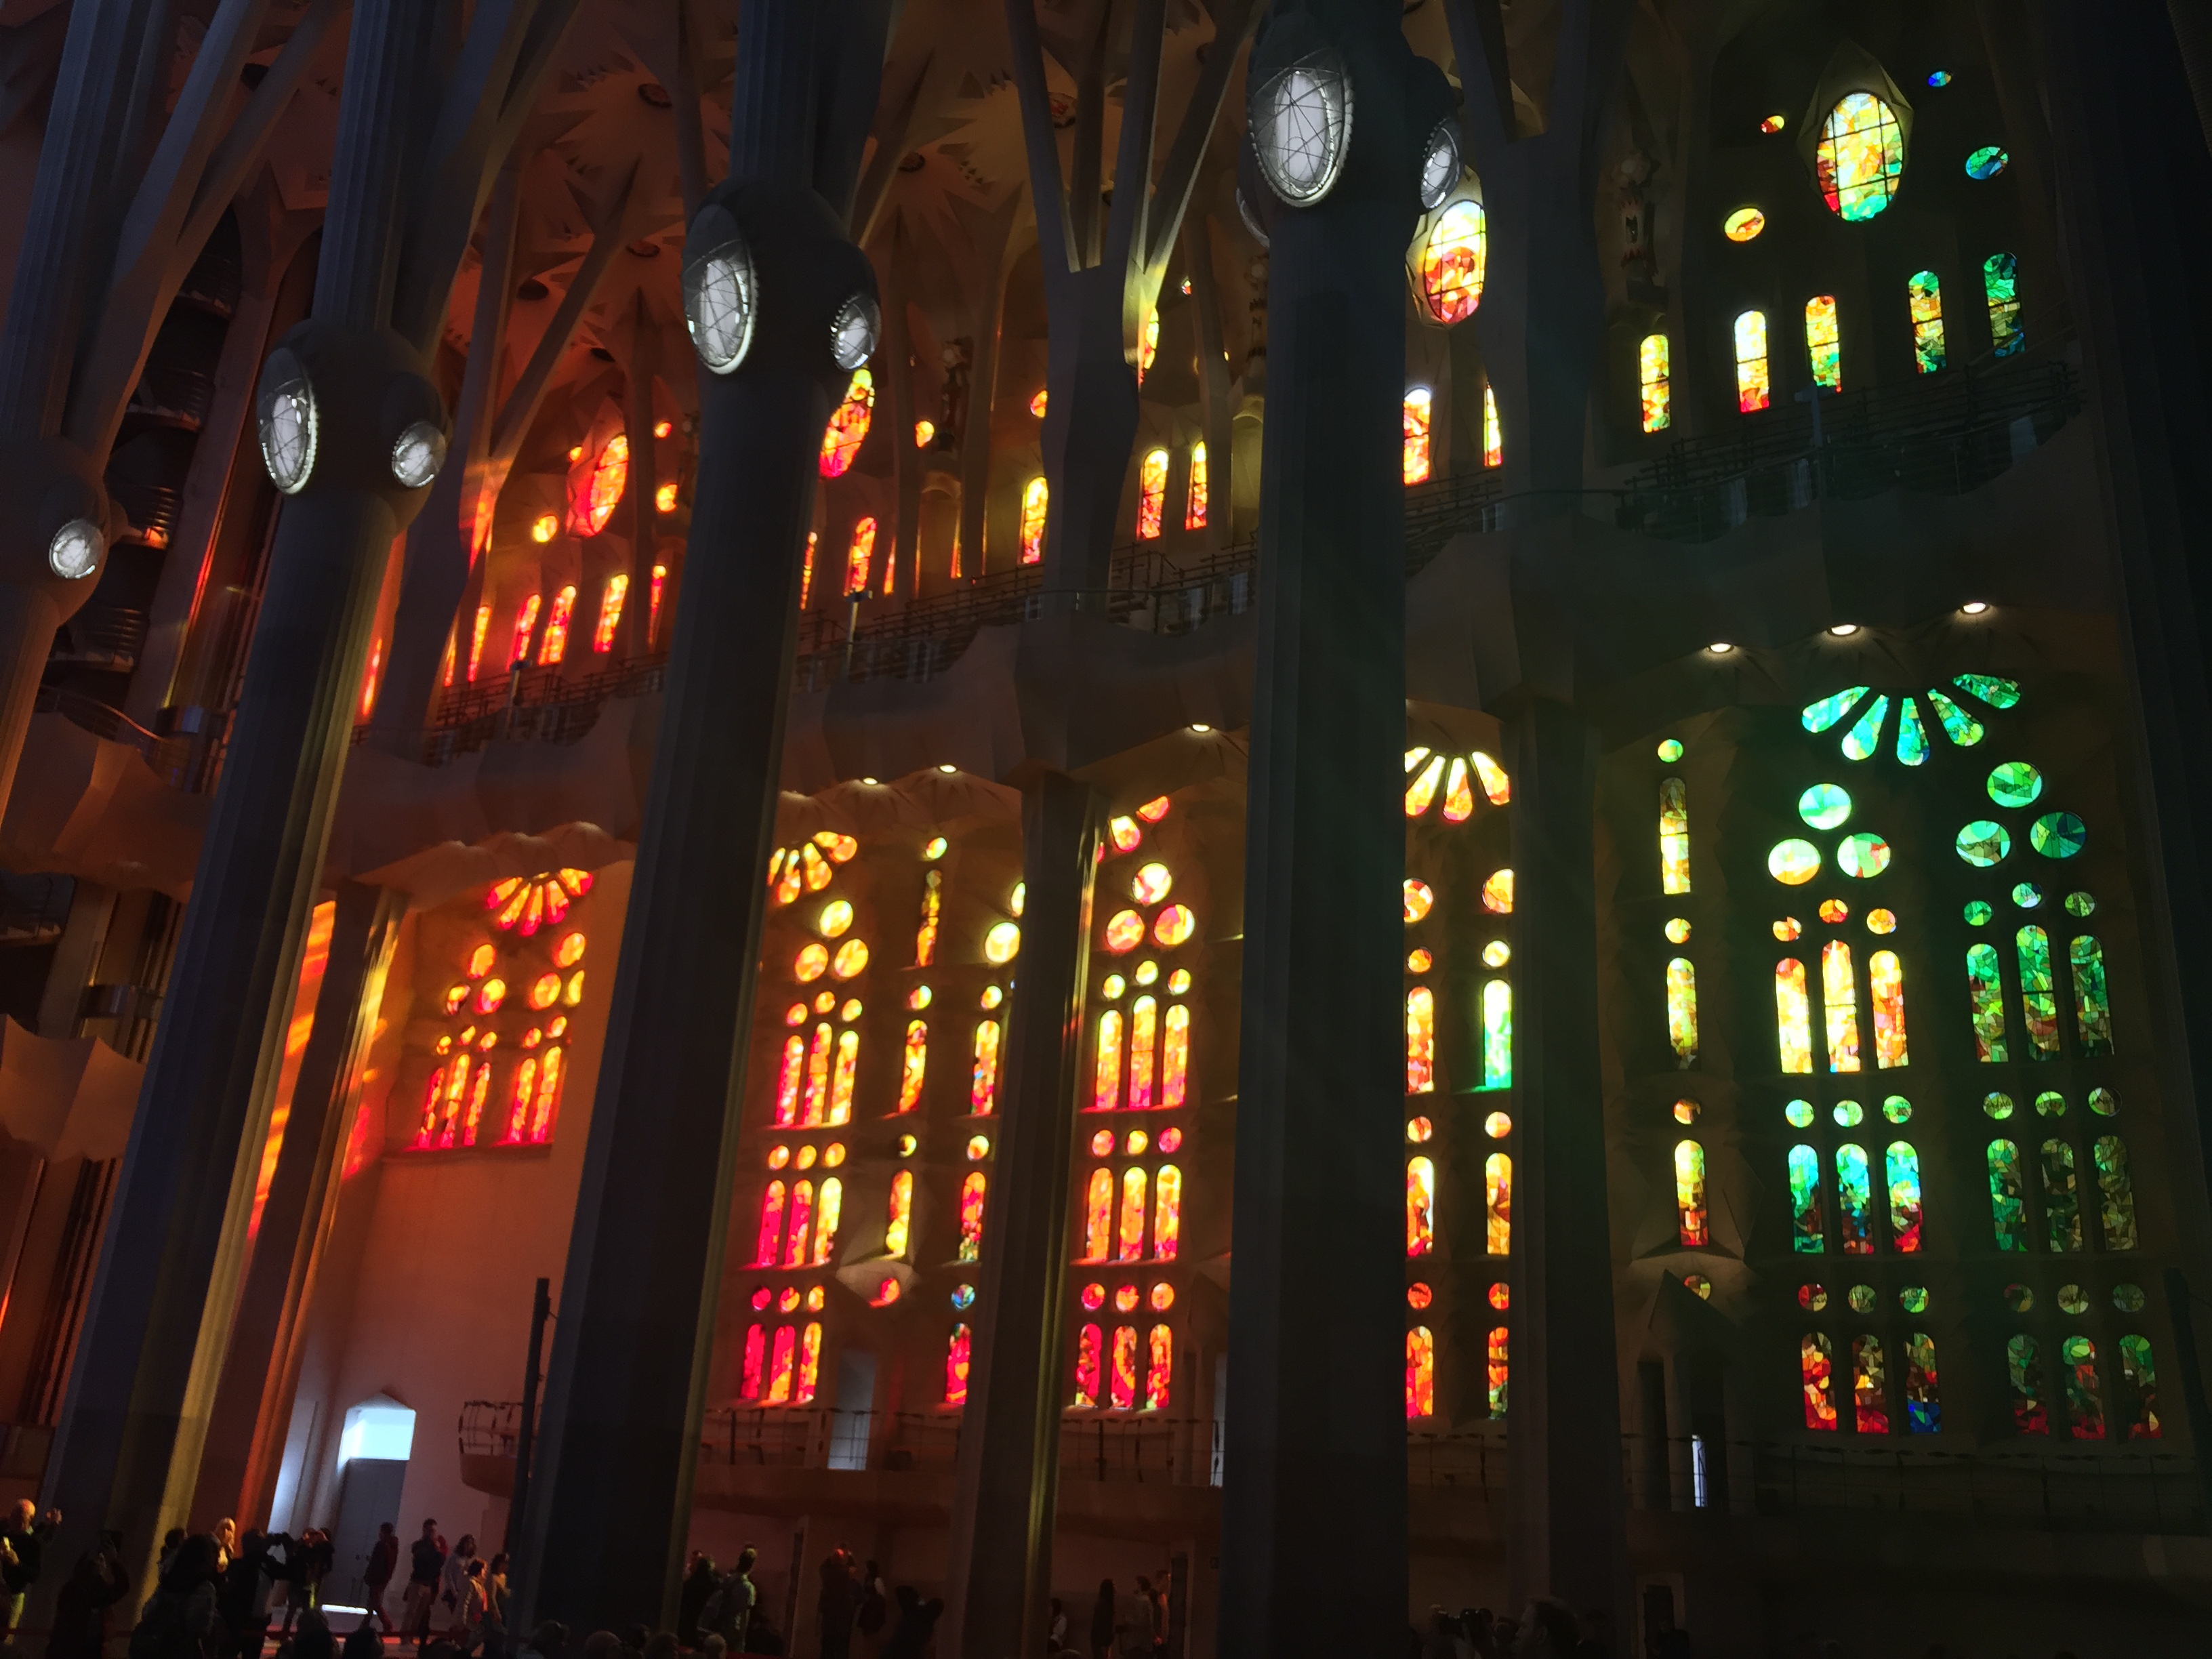
\includegraphics[width=.35\textwidth]{images/IMG_3267.JPG}};
		\node[inner sep=5pt] (sagrada2) at (10,0)
		{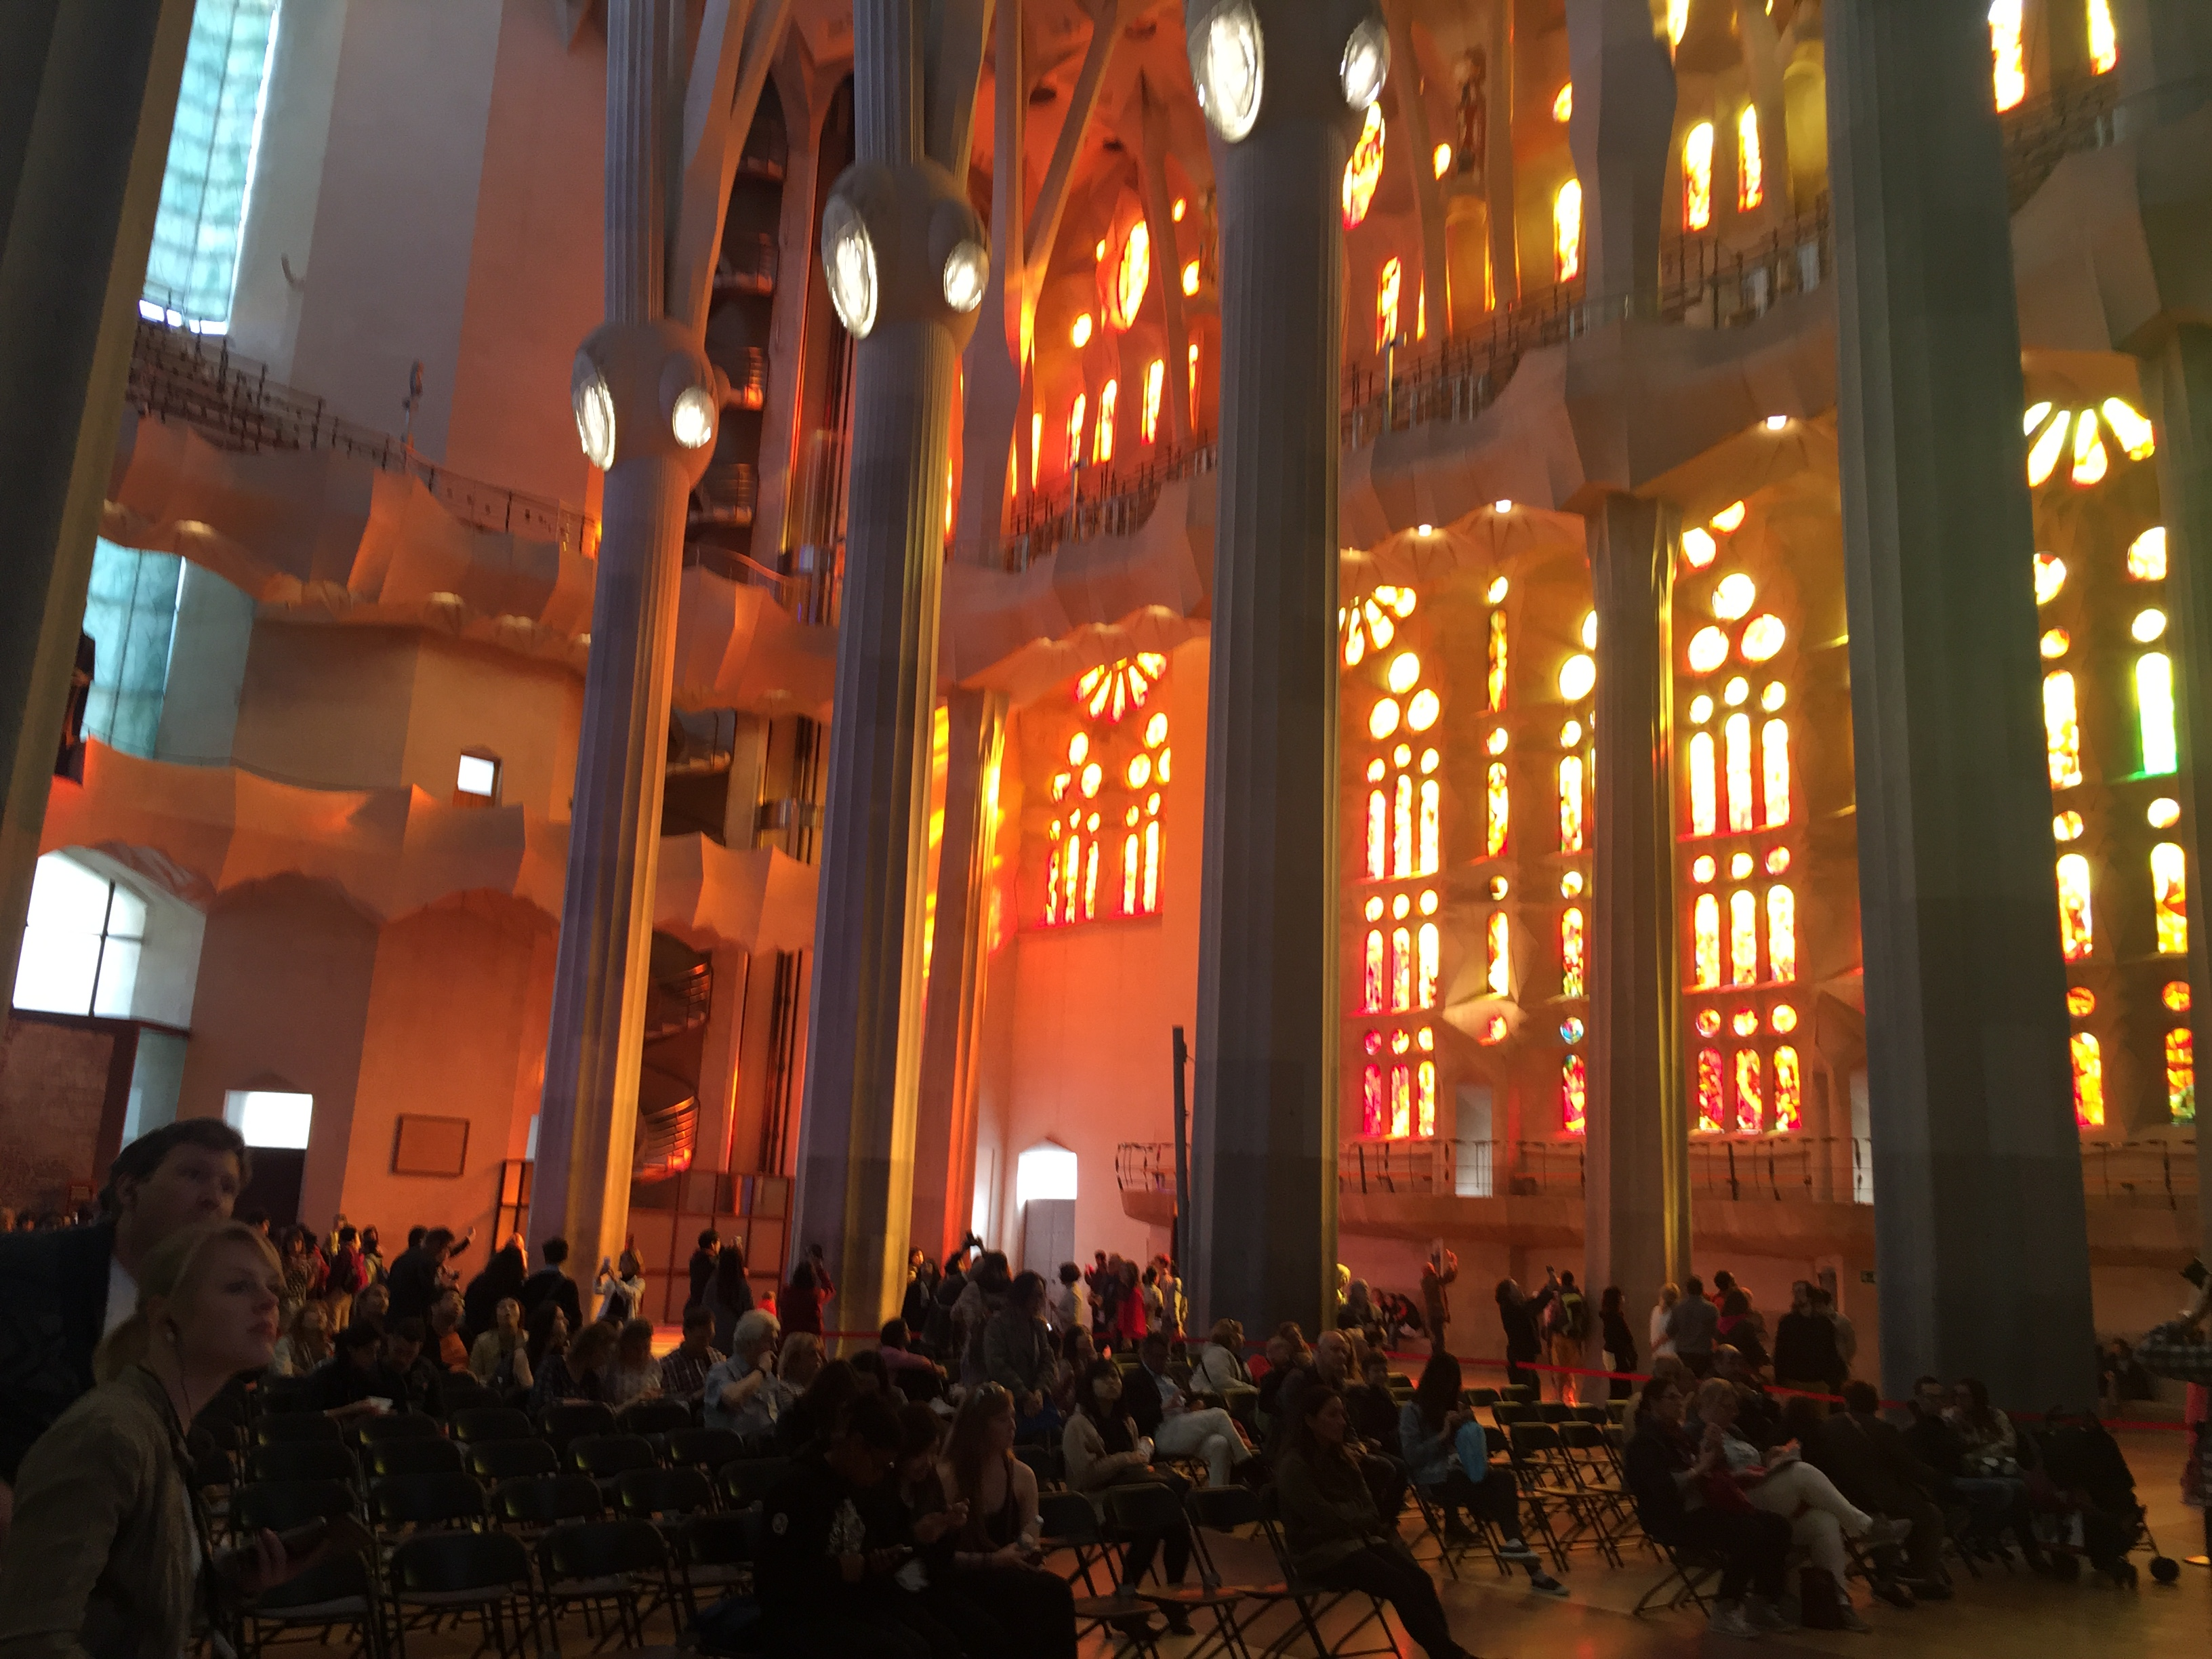
\includegraphics[width=.35\textwidth]{images/IMG_3268.JPG}};
		
		\node[inner sep=5pt] (graph1) at (0,-6)
		{
			\begin{tikzpicture}
			\node[draw, circle, fill=graphc2] (n1) at (0,-1) {};
			\node[draw, circle, fill=graphc3] (n2) at (1,-0.67) {};
			\node[draw, circle, fill=graphc4] (n3) at (2,-0.33) {};
			\node[draw, circle, fill=graphc2] (n4) at (0,-2) {};
			\node[draw, circle, fill=graphc3] (n5) at (1,-1.9) {};
			\node[draw, circle, fill=graphc4] (n6) at (2,-1.8) {};
			
			\draw[<->] (n1) -- (n2);
			\draw[<->] (n2) -- (n3);
			\draw[<->] (n1) -- (n4);
			\draw[<->] (n2) -- (n5);
			\draw[<->] (n4) -- (n5);
			\draw[<->] (n5) -- (n6);
			\end{tikzpicture}
		};
		
		\node[inner sep=5pt] (graph2) at (10,-6)
		{
			\begin{tikzpicture}
			\node[draw, circle] (n0) at (-1,-1.5) {};
			\node[draw, circle, fill=graphc1] (n7) at (-0.8,-0.33) {};
			\node[draw, circle, fill=graphc2] (n1) at (0,-1) {};
			\node[draw, circle, fill=graphc3] (n2) at (1,-0.67) {};
			\node[draw, circle, fill=graphc2] (n4) at (0,-2) {};
			\node[draw, circle, fill=graphc3] (n5) at (1,-1.9) {};
			
			\draw[<->] (n0) -- (n1);
			\draw[<->] (n0) -- (n4);
			\draw[<->] (n0) -- (n7);
			\draw[<->] (n1) -- (n2);
			\draw[<->] (n1) -- (n4);
			\draw[<->] (n2) -- (n5);
			\draw[<->] (n4) -- (n5);
			\end{tikzpicture}
		};
		
		\draw[->,thick] (sagrada1.east) -- (sagrada2.west)
		node[midway,fill=white] {Similarity};
		\draw[->,thick] (graph1.east) -- (graph2.west)
		node[midway,fill=white] {Similarity};
		
		\draw[->,thick] (sagrada1.south) -- (graph1.north)
		node[midway,fill=white] {Transform};
		\draw[->,thick] (sagrada2.south) -- (graph2.north)
		node[midway,fill=white] {Transform};
	\end{tikzpicture}
}
\caption{An example of the expected similarity between two views of the same scene. Similar objects and scenes should theoretically generate similar graphs after a suitable transformation, enabling recognition across images.\label{fig:intro-sim}}
\end{figure}

%====================================================
\section{Graphs, Search and Similarity}
\label{sec:graph-search}
%====================================================

%?? Graph definitions etc
First, we must define graphs more precisely.
An undirected graph $\mathcal{G}$ may be written $\mathcal{G} = (V,E)$ for a vertex set $V$ and an edge set $E \subseteq \lbrace \lbrace u,v \rbrace : u,v \in V \rbrace $, i.e.\ each edge $e \in E$ is a set of two vertices from $V$.
To access these sets, I define the functions $\operatorname{V}(\mathcal{G})=V$ and $\operatorname{E}(\mathcal{G})=E$ to retrieve the vertex and edge set respectively.
For some $u,v \in V$, we may write $u \sim_\mathcal{G} v$ to mean $u$ and $v$ are adjacent vertices in $\mathcal{G}$ ($\lbrace u,v \rbrace \in E$), and use $N_\mathcal{G}(u)$ to refer to $u$'s \emph{neighbourhood}---the set of all vertices in $V \backslash \lbrace u \rbrace$ adjacent to $u$ in $\mathcal{G}$.
This definition allows loops, e.g.\ $u \sim_\mathcal{G} u$ with the caveat that $u \notin N_\mathcal{G}(u)$.
Additionally, the \emph{order} of $\mathcal{G}$ refers to the count of $\mathcal{G}$'s vertices ($\operatorname{Ord}(\mathcal{G})=|V|$), and the \emph{size} of $\mathcal{G}$ refers to the count of $\mathcal{G}$'s edges ($\operatorname{Sz}(\mathcal{G})=|E|$).
Where $\mathcal{G}$ is clear from context, the relevant subscripts will be elided.

The graphs produced by the techniques I outline are \emph{attributed undirected multigraphs}: vertices and edges may have labels, and each pair of vertices may share multiple edges.
Given domains $L_v, L_e$ for vertex and edge labels respectively, we redefine $\mathcal{G} = (V,E,\ell_v,\ell_e)$ for a vertex set $V$, an edge set $E$, a vertex label mapping $\ell_v: V \rightarrow L_v$ and an edge mapping $\ell_e: E \rightarrow \lbrace(\lbrace u,v \rbrace, l): u,v \in V, l \in L_e\rbrace$.
%For any vertex $v \in V$, its label in $\mathcal{G}$ is given as $l_\mathcal{G}(v)$.
We can succinctly describe the edges between any $u, v \in V$ with a sorted (non-decreasing) sequence of labels, $\operatorname{seq}_\mathcal{G}(u, v)$.
This allows us to define basic adjacency, and thus the basic neighbourhood: $u \sim_\mathcal{G} v \iff |\operatorname{seq}_\mathcal{G}(u,v)| \ge 1$.
For matching such graphs, we require three new neighbourhood definitions.
Given a sorted label sequence $s$, we may define the \emph{exact neighbourhood} $N^{=}_{s,\mathcal{G}}(u)$ as the set of all $v \in N_\mathcal{G}(u)$ such that $\operatorname{seq}_\mathcal{G}(u,v)=s$.
The \emph{sufficient neighbourhood} $N^{\succcurlyeq}_{s,\mathcal{G}}(u)$ is the set of all $v \in N_\mathcal{G}(u)$ where we may map each label in $s$ to a distinct label of equal value in $\operatorname{seq}_\mathcal{G}(u,v)$---we say that $s \preccurlyeq \operatorname{seq}_\mathcal{G}(u,v)$ if such a mapping exists.
Finally, the \emph{overlap neighbourhood} $N^{\circ}_{s,\mathcal{G}}(u)$ is the set of all $v \in N_\mathcal{G}(u)$ where at least one label in $s$ may be mapped to a label of equal value in $\operatorname{seq}_\mathcal{G}(u,v)$.
%=\lbrace v \in V \backslash \lbrace u \rbrace: \operatorname{seq}_\mathcal{G}(u,v)=s\rbrace$
For simplicity, I shall define the core search and similarity problems using undirected graphs.

Transformation from an image to a graph will create a graph whose structure corresponds to the image's content and invariants.
If an image $I$ contains an object, it is thus reasonable to assume that the graph produced from an image of only that object should be reproduced within $I$'s graph model---this may be useful when e.g., searching for a road sign in a view seen by an autonomous car.
This form of graph search is known as the \emph{subgraph isomorphism problem} (SIP), which is concerned with finding the exact structure of some pattern graph $\mathcal{P}=(V_\mathcal{P}, E_\mathcal{P})$ within a target graph $\mathcal{T}=(V_\mathcal{T}, E_\mathcal{T})$---an example is provided in \cref{fig:lit-sip}.
More precisely, for the non-induced variant of SIP the problem is to find an injective mapping $i : V_\mathcal{P} \rightarrow V_\mathcal{T}$ such that $\forall u,v \in V_\mathcal{P}, i(u) \neq i(v)$ and $u \sim_\mathcal{P} v \Rightarrow i(u) \sim_\mathcal{T} i(v)$, preserving adjacency and ensuring no two vertices of $\mathcal{P}$ are mapped to the same vertex of $\mathcal{T}$.
The induced variant additionally imposes that $\forall u,v \in V_\mathcal{P}, u \nsim_\mathcal{P} v \Rightarrow i(u) \nsim_\mathcal{T} i(v)$, ensuring that non-adjacent vertices in $\mathcal{P}$ must remain non-adjacent in the embedding in $\mathcal{T}$.
While SIP is \NP-Complete \cite{Cook-SAT-SIP-NP, Computers-and-Intractibility}, with modern algorithms such as \citeauthor{SIP-Glasgow}'s Glasgow solver it is computationally feasible for graphs on the order of several thousand vertices \cite{SIP-Glasgow}.
Trends in recent work have focused on increasing performance for larger instances through more costly filtering and pre-processing \cite{SIP-LAD, SIP-SND, SIP-Glasgow}---for this reason, older approaches such as VF2 \cite{SIP-VF2} remain competitive on smaller instances \cite{SIP-Hard-Instances}.
%The constraint programming 
%?? SIP \cite{SIP-VF2, SIP-LAD, SIP-SND, SIP-Glasgow}, Regin filtering \cite{AllDiff}, Complexity \cite{Cook-SAT-SIP-NP}

\begin{figure}
	\centering
	\resizebox{\columnwidth}{!}{
	\begin{tikzpicture}
	
	\node[label=below:{$\mathcal{P}$}] (p) at (0,0){
		\begin{tikzpicture}[scale=1]
		\begin{scope}[auto, every node/.style={draw,circle,minimum size=2em,inner sep=1},node distance=2cm]
		\node[draw, circle] (n1) at (0,0) {a};
		\node[draw, circle] (n2) at (0,-1) {c};
		\node[draw, circle] (n3) at (1,0) {b};
		\node[draw, circle] (n4) at (1,-1) {d};
		\end{scope}
		
		\draw[-] (n1) -- (n3);
		\draw[-] (n2) -- (n4);
		\draw[-] (n1) -- (n4);
		\draw[-] (n2) -- (n3);
		\draw[-] (n3) -- (n4);
		\end{tikzpicture}
	};
	
	\node[label=below:{$\mathcal{T}$}] (t) at (4,0){
		\begin{tikzpicture}[scale=1]
		\begin{scope}[auto, every node/.style={draw,circle,minimum size=2em,inner sep=1},node distance=2cm]
		\node[draw, circle] (n1) at (2,0) {2};
		\node[draw, circle] (n2) at (0,-1) {4};
		\node[draw, circle] (n3) at (1,0) {1};
		\node[draw, circle] (n4) at (1,-1) {5};
		
		\node[draw, circle] (n5) at (2,-1) {6};
		\node[draw, circle] (n6) at (3,0) {3};
		\end{scope}
		
		\draw[-] (n1) -- (n3);
		\draw[-] (n2) -- (n4);
		\draw[-] (n1) -- (n4);
		\draw[-] (n2) -- (n3);
		\draw[-] (n3) -- (n4);
		
		\draw[-] (n5) -- (n6);
		\draw[-] (n1) -- (n6);
		\draw[-] (n3) -- (n5);
		\end{tikzpicture}
	};
	
	\node[label=below:{Embedding}] (em) at (9,0){
		\begin{tikzpicture}[scale=1]
		\begin{scope}[auto, every node/.style={draw,circle,minimum size=2em,inner sep=1},node distance=2cm]
		\node[draw, circle, fill=uofgpumpkin] (n1) at (2,0) {2};
		\node[draw, circle, fill=uofgpumpkin] (n2) at (0,-1) {4};
		\node[draw, circle, fill=uofgpumpkin] (n3) at (1,0) {1};
		\node[draw, circle, fill=uofgpumpkin] (n4) at (1,-1) {5};
		
		\node[draw, circle] (n5) at (2,-1) {6};
		\node[draw, circle] (n6) at (3,0) {3};
		\end{scope}
		
		\draw[-, color=uofgpumpkin] (n1) -- (n3);
		\draw[-, color=uofgpumpkin] (n2) -- (n4);
		\draw[-, color=uofgpumpkin] (n1) -- (n4);
		\draw[-, color=uofgpumpkin] (n2) -- (n3);
		\draw[-, color=uofgpumpkin] (n3) -- (n4);
		
		\draw[-] (n5) -- (n6);
		\draw[-] (n1) -- (n6);
		\draw[-] (n3) -- (n5);
		\end{tikzpicture}
	};
	
	\draw[->, thick] (t) -- (em);
	
\end{tikzpicture}
}
\caption{
		An example of the subgraph isomorphism problem between two graphs $\mathcal{P}$ and $\mathcal{T}$.
		$\mathcal{P}$'s embedding within $\mathcal{T}$ is highlighted in orange---this is a valid matching in both the induced and non-induced SIP variants.
		\label{fig:lit-sip}
}
\end{figure}

%?? MCS \cite{Between-MCS-SIP}, James+Ciaran+Pat's new paper too \cite{MCS-McSplit}, complexity \cite[p.\ 74--75]{Computers-and-Intractibility}
In reality, elements of an object's graph structure may not be reproduced in the graph of an embedding due to either occlusion, image distortion or object scale.
In this case, it is worthwhile to examine how much two image graphs have in common to identify common elements and substructures.
Between two graphs $\mathcal{P}$ and $\mathcal{T}$ this is known as the \emph{maximum common subgraph problem} (MCS), which is the search for the largest subgraph of $\mathcal{P}$ which is isomorphic to some subgraph of $\mathcal{T}$ as in SIP.
\Cref{fig:lit-mcs} offers an example instance.
While this problem as described is \NP-Hard, it is considerably harder in practice than SIP---the current state-of-the-art, McSplit, can operate on graphs of order 35--40 \cite{MCS-McSplit}, where other approaches are limited to around 30 vertices.
Even so, this approach applies only to the induced variant of MCS and largely prevents the addition of side constraints.
For such flexibility we must consider either $k\downarrow$ \cite{Between-MCS-SIP}, a repeated application of the Glasgow SIP solver excluding $k$ vertices, or a max-clique-based approach using the \emph{association graph encoding} \cite{MCS-Clique-CP}.
In this regard there is a trade-off to be made: while the clique-based approach still achieves the best performance on labelled instances \cite{MCS-McSplit}, $k\downarrow$ requires far less memory to process high-order graphs.
I choose to examine and modify $k\downarrow$ for these reasons, but this still requires that the order of any graphs must remain small to perform occlusion-robust matching with this technique.

By computing similar structures between any two graphs as above, we may then quantify how similar they are by considering the order of the MCS.
This is in turn a key part of establishing how \emph{dissimilar} a pair of graphs are, and given that MCS order does not take into account the sizes of $\mathcal{P}$ or $\mathcal{T}$ such a metric is more desirable for global classification.
We may then use the MCS to compute the number of discrete changes needed to transform $\mathcal{P}$ into $\mathcal{T}$---the \emph{graph edit distance} (GED) \cite{GraphEditDist-MCS}.
For classification purposes, I consider a simplified expression which disregards edge costs:
$$ \operatorname{GED}(\mathcal{P}, \mathcal{T}) = \operatorname{Ord}(\mathcal{P}) + \operatorname{Ord}(\mathcal{T}) - 2 \operatorname{Ord}(\operatorname{MCS}(\mathcal{P}, \mathcal{T})) $$

\begin{figure}
	\centering
	\resizebox{0.8\columnwidth}{!}{
	\begin{tikzpicture}
	
	\node[label=below:{$\mathcal{P}$}] (p) at (0,0){
		\begin{tikzpicture}[scale=1]
		\begin{scope}[auto, every node/.style={minimum size=2em,inner sep=1},node distance=2cm]
		\node[draw, circle] (n1) at (0,0) {a};
		\node[draw, circle] (n2) at (0,-1) {c};
		\node[draw, circle] (n3) at (1,0) {b};
		\node[draw, circle] (n4) at (1,-1) {d};
		
		\draw[-] (n1) -- (n3);
		\draw[-] (n2) -- (n4);
		\draw[-] (n1) -- (n4);
		\draw[-] (n2) -- (n3);
		\draw[-] (n3) -- (n4);
		\end{scope}
		\end{tikzpicture}
	};
	
	\node[label=below:{$\mathcal{T}$}] (t) at (3,0){
		\begin{tikzpicture}[scale=1]
		\begin{scope}[auto, every node/.style={draw,circle,minimum size=2em,inner sep=1},node distance=2cm]
		\node[draw, circle] (n1) at (0,0) {1};
		\node[draw, circle] (n2) at (0,-1) {3};
		\node[draw, circle] (n3) at (1,0) {2};
		\node[draw, circle] (n4) at (1,-1) {4};
		\end{scope}
		
		\draw[-] (n1) -- (n3);
		\draw[-] (n2) -- (n4);
		\draw[-] (n1) -- (n2);
		\draw[-] (n2) -- (n3);
		\draw[-] (n3) -- (n4);
		
		\end{tikzpicture}
	};
	
	\node[label=below:{Embedding}] (em) at (7,0){
		\begin{tikzpicture}[scale=1]
		\begin{scope}[auto, every node/.style={draw,circle,minimum size=2em,inner sep=1},node distance=2cm]
		\node[draw, circle] (n1) at (0,0) {a};
		\node[draw, circle, fill=uofgpumpkin] (n2) at (0,-1) {c};
		\node[draw, circle, fill=uofgpumpkin] (n3) at (1,0) {b};
		\node[draw, circle, fill=uofgpumpkin] (n4) at (1,-1) {d};
		
		\draw[-] (n1) -- (n3);
		\draw[-, color=uofgpumpkin] (n2) -- (n4);
		\draw[-] (n1) -- (n4);
		\draw[-, color=uofgpumpkin] (n2) -- (n3);
		\draw[-, color=uofgpumpkin] (n3) -- (n4);
		
		\node[draw, circle] (n1') at (2,0) {1};
		\node[draw, circle, fill=uofgpumpkin] (n2') at (2,-1) {3};
		\node[draw, circle, fill=uofgpumpkin] (n3') at (3,0) {2};
		\node[draw, circle, fill=uofgpumpkin] (n4') at (3,-1) {4};
		
		
		\draw[-] (n1') -- (n3');
		\draw[-, color=uofgpumpkin] (n2') -- (n4');
		\draw[-] (n1') -- (n2');
		\draw[-, color=uofgpumpkin] (n2') -- (n3');
		\draw[-, color=uofgpumpkin] (n3') -- (n4');
		\end{scope}
		\end{tikzpicture}
	};
	
	\draw[->, thick] (t) -- (em);
	
\end{tikzpicture}
}
\caption{
		An example of the maximum common subgraph problem between two graphs $\mathcal{P}$ and $\mathcal{T}$.
		The MCS's embedding within both $\mathcal{P}$ and $\mathcal{T}$ is highlighted in orange.
		Note that this embedding is not unique, although for this choice of $\mathcal{P}$ and $\mathcal{T}$ the MCS itself is.
		\label{fig:lit-mcs}
}
\end{figure}

%====================================================
\section{On Existing Image Graph Models}
\label{sec:image-weakness}
%====================================================

%\citeauthor{Plane-Graphs-From-Images} \cite{Plane-Graphs-From-Images}

%?? Approaches such as seen in \cite{Submap-Iso-Images} use Delaunay -- Enhanced by structural cues such as in \cite{Plane-Graphs-From-Images}

\begin{figure*}
	\centering
	\begin{subfigure}[b]{0.22\textwidth}
		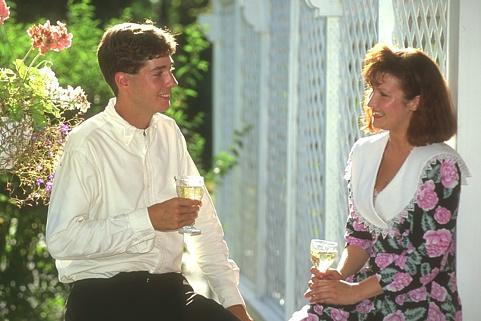
\includegraphics[width=\textwidth]{images/bsd-157055}
		\caption{BSD test image}
		\label{fig:explor-bsd}
	\end{subfigure}
	~
	\begin{subfigure}[b]{0.35\textwidth}
		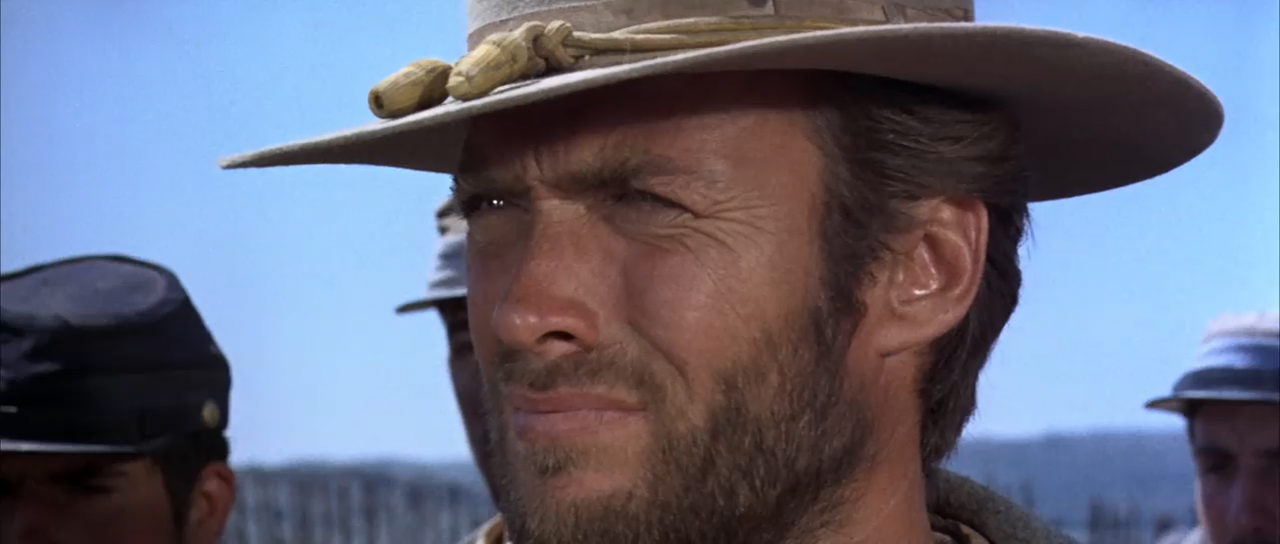
\includegraphics[width=\textwidth]{images/gbu2}
		\caption{Film frame 1}
		\label{fig:explor-ff1}
	\end{subfigure}
	~
	\begin{subfigure}[b]{0.35\textwidth}
		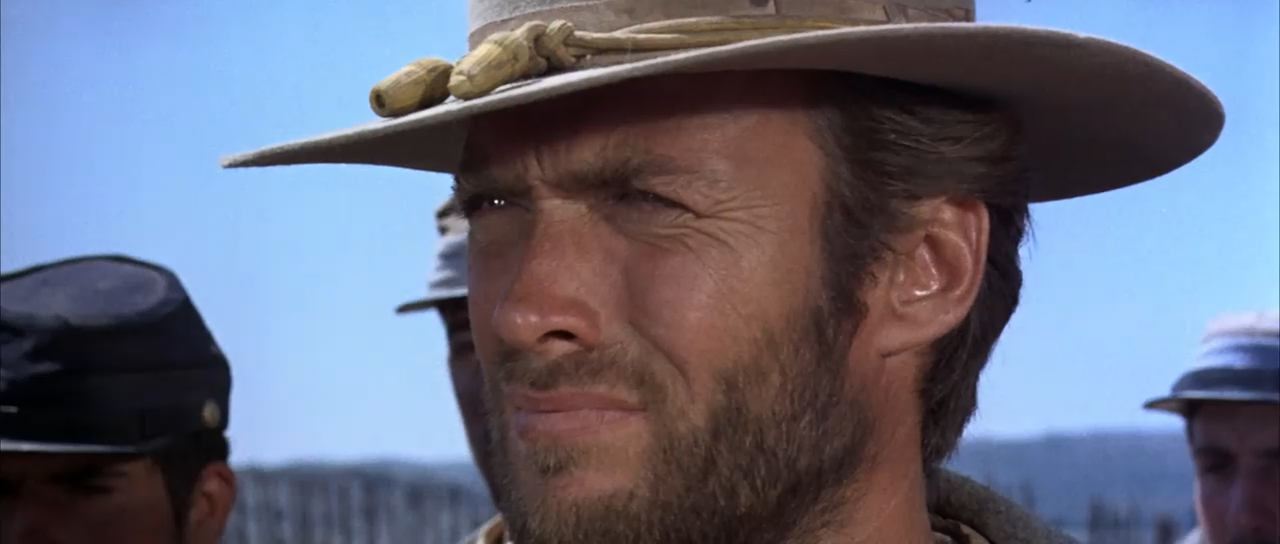
\includegraphics[width=\textwidth]{images/gbu3}
		\caption{Film frame 2}
		\label{fig:explor-ff2}
	\end{subfigure}
	
	\vspace{0.5em}
	
	\caption{
		Images used for evaluation of \citeauthor{Plane-Graphs-From-Images}'s \cite{Plane-Graphs-From-Images} approach.
	}
\end{figure*}

\begin{figure*}
	\centering
	\begin{subfigure}[b]{0.22\textwidth}
		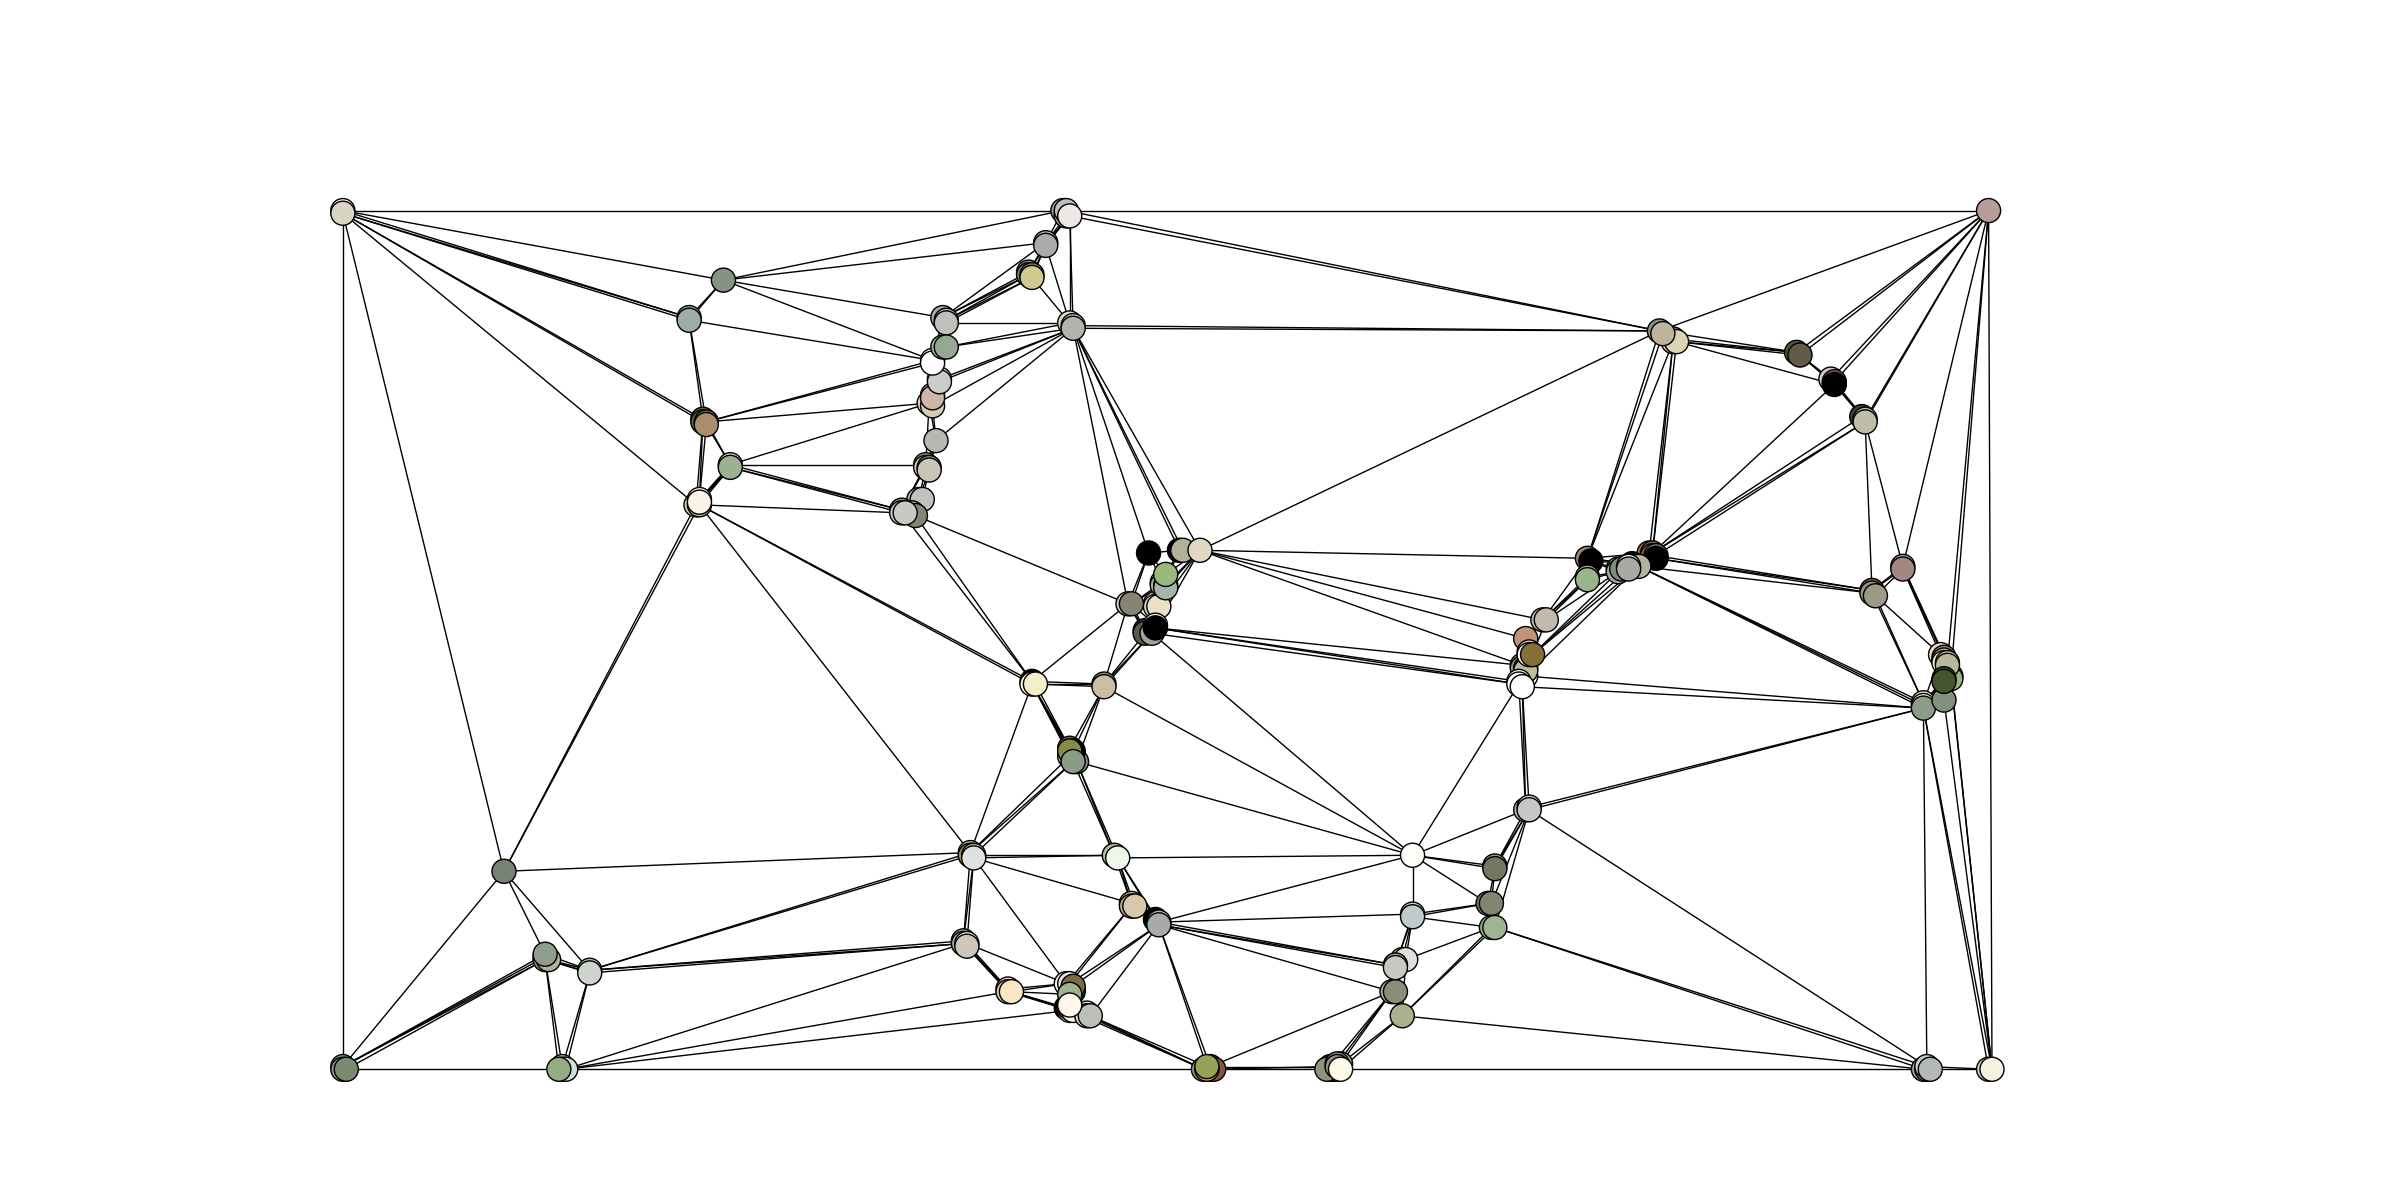
\includegraphics[width=\textwidth]{img-results/nrm}
		\caption{
				BSD test image, normal.
				$|V|=245$, $|E|=707$.
		}
		\label{fig:explor-bsdnrmgraph}
	\end{subfigure}
	~
	\begin{subfigure}[b]{0.22\textwidth}
		
\includegraphics[width=\textwidth]{img-results/180}
		\caption{
				BSD test image, \SI{180}{\degree} rotation.
				$|V|=247$, $|E|=705$.
		}
		\label{fig:explor-bsd180graph}
	\end{subfigure}
	~
	\begin{subfigure}[b]{0.22\textwidth}
		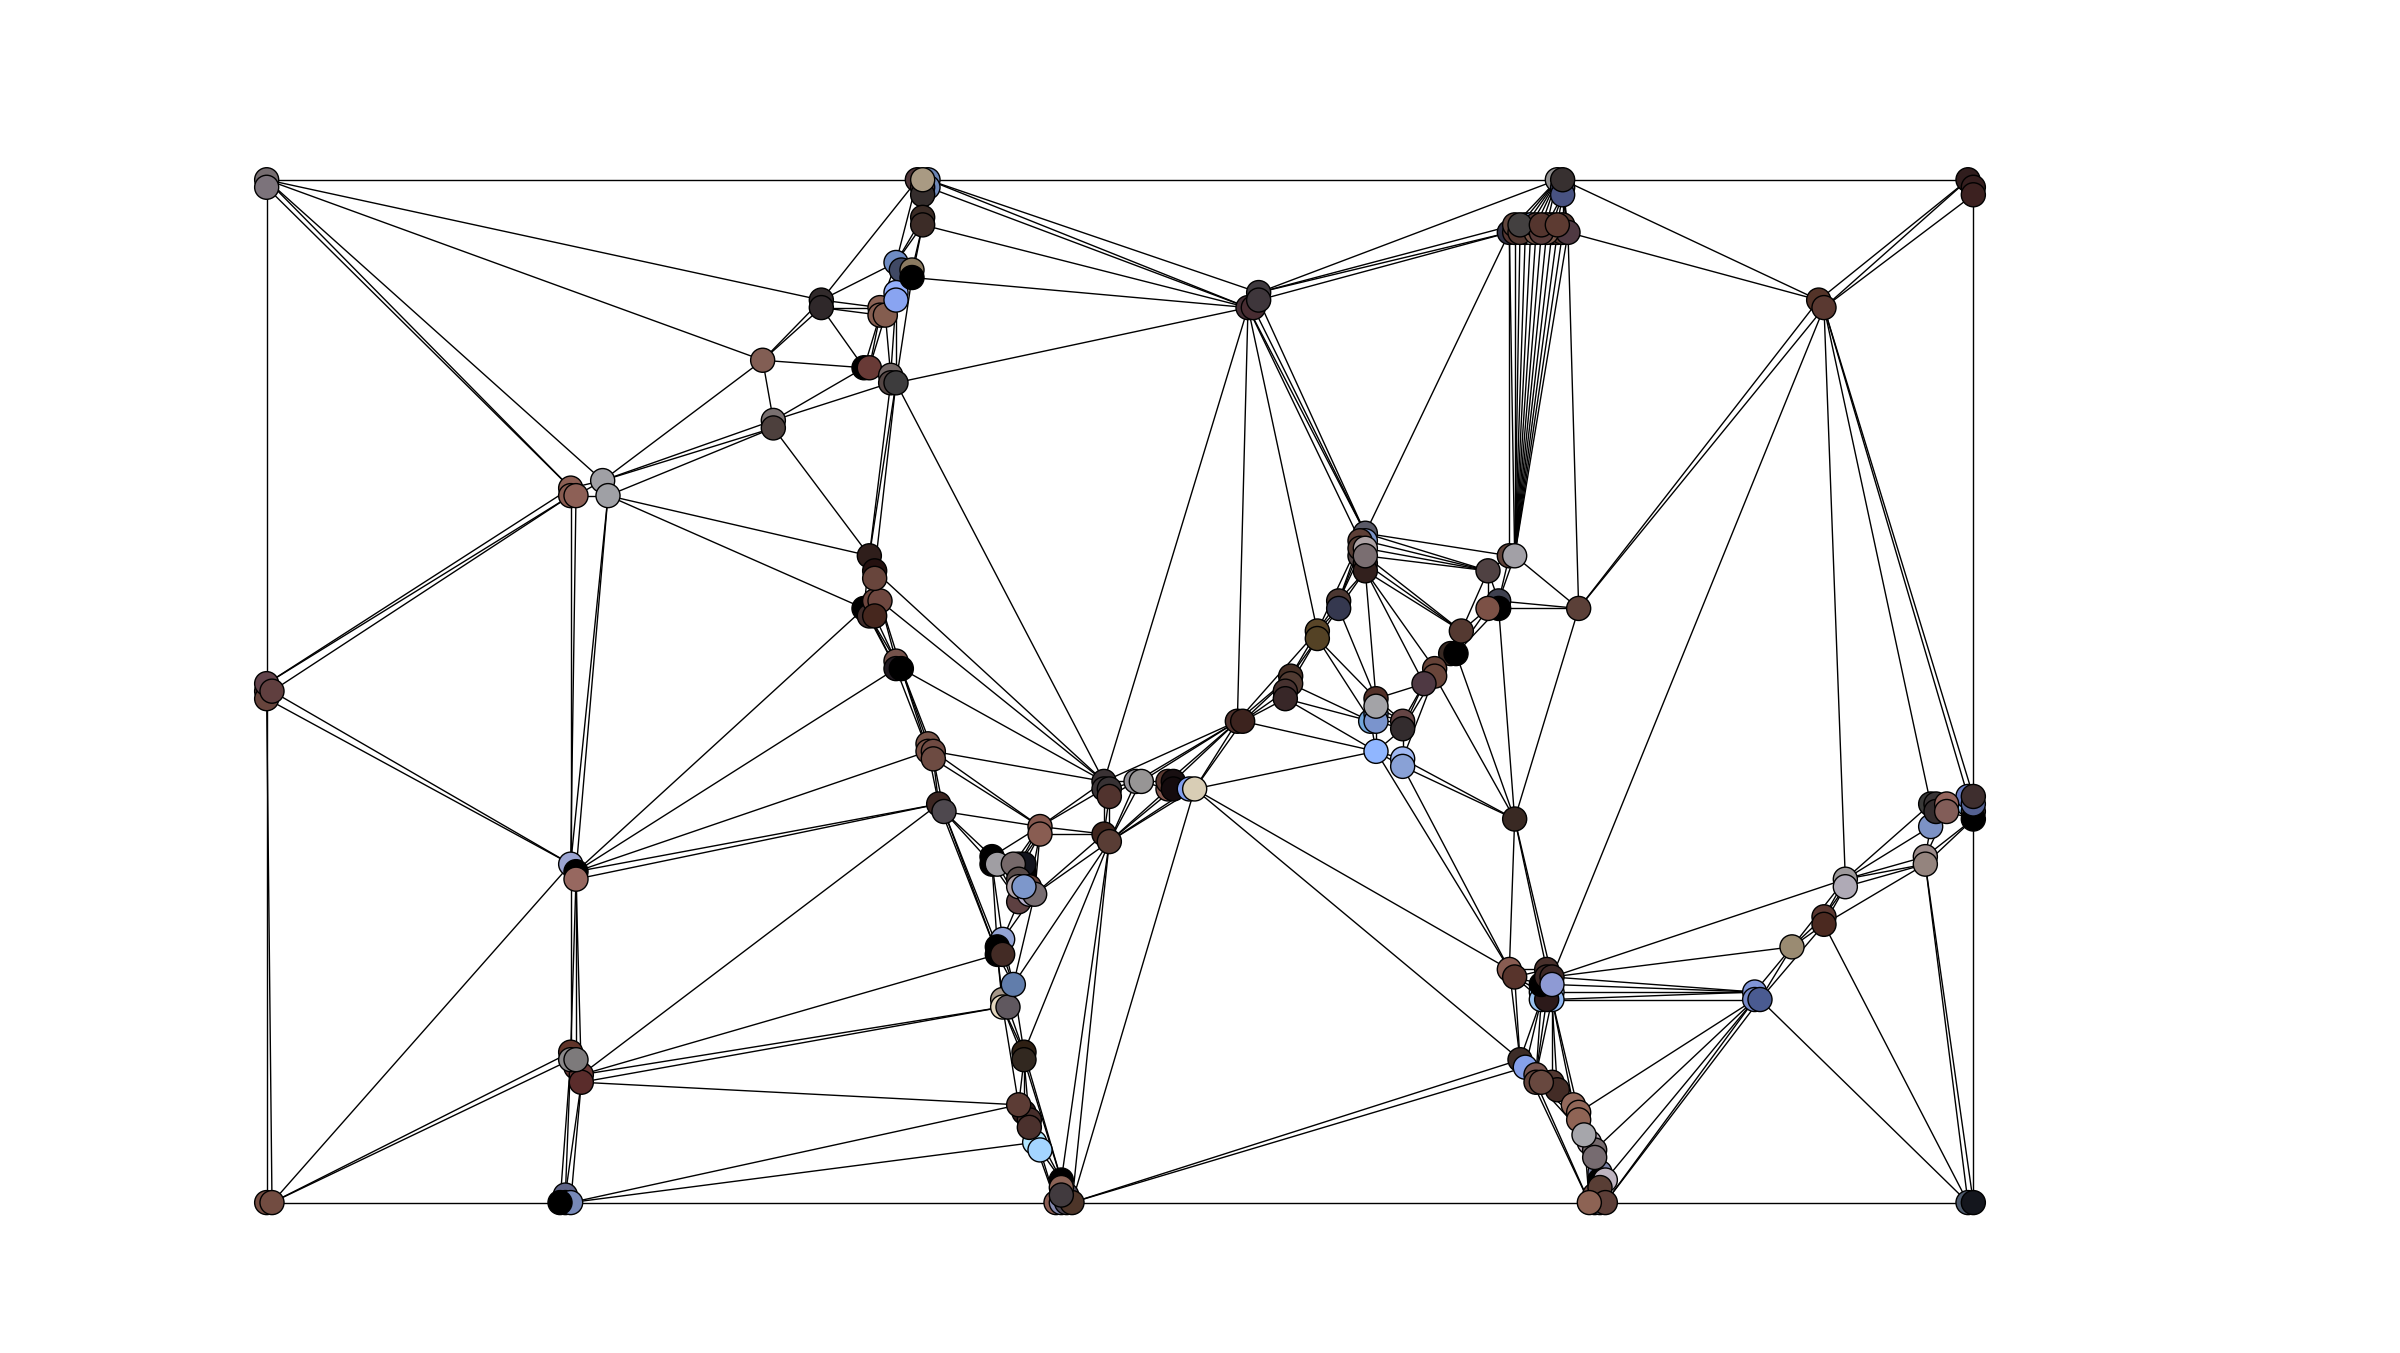
\includegraphics[width=\textwidth]{img-results/gbu-smr2-graph}
		\caption{
				Film frame 1.
				$|V|=264$, $|E|=755$.
		}
		\label{fig:explor-ff1graph}
	\end{subfigure}
	~
	\begin{subfigure}[b]{0.22\textwidth}
		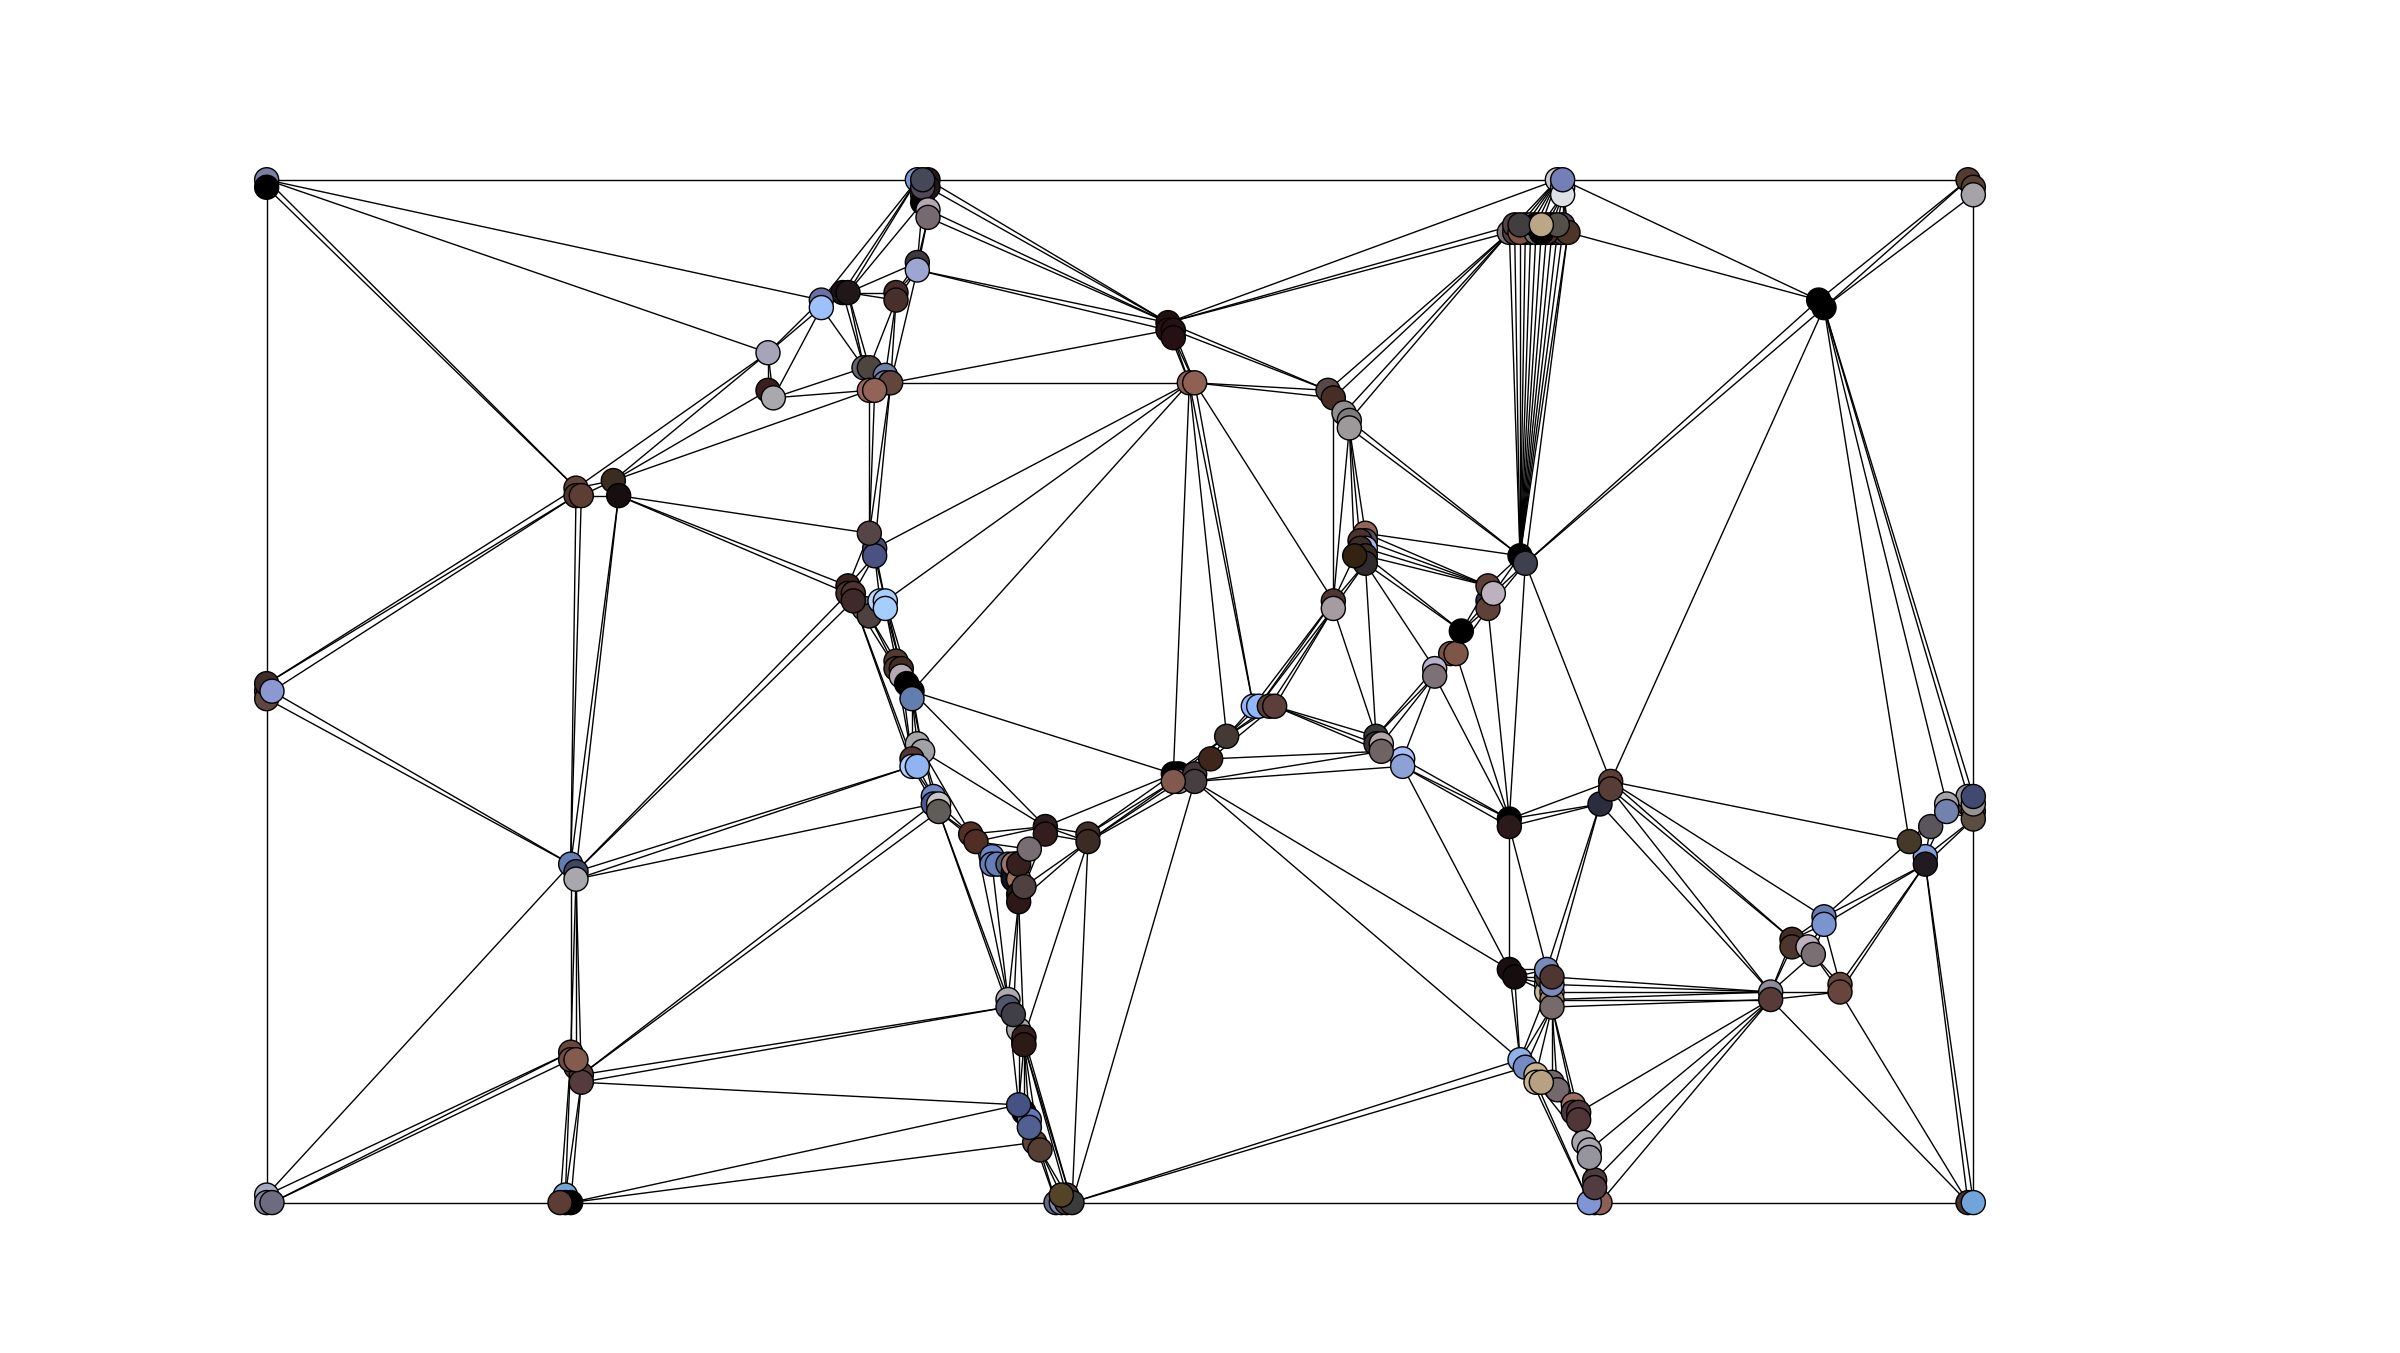
\includegraphics[width=\textwidth]{img-results/gbu-smr3-graph}
		\caption{
				Film frame 2.
				$|V|=260$, $|E|=743$.
		}
		\label{fig:explor-ff2graph}
	\end{subfigure}
	
	\vspace{0.5em}
	
	\caption{
		Graph output after boundary walking and Delaunay triangulation.
		$|V|$ and $|E|$ denote the vertex count and edge count, respectively.
	}
\end{figure*}

For graph modelling of generic images, present techniques typically build graphs by applying the \emph{Delaunay triangulation} \cite{Delaunay} to a set of interest pixels located within an image.
This process places edges between vertices with coordinate labels to construct a face-connected plane graph; specifically, where each face is a triangle.
Crucially, this mesh is subject to one key criterion designed to minimise the incidence of sliver triangles: no point may lie inside the circumcircle of any produced triangle.
Efficient algorithms exist for its computation \cite{DelaunayAlgs,DelaunayModern}.
This avenue is explored briefly by \citeauthor{Submap-Iso-Images} \cite{Submap-Iso-Images}, and expanded upon by \citeauthor{Plane-Graphs-From-Images} to make use of structural cues provided by image segmentation algorithms \cite{Plane-Graphs-From-Images}.
The authors of these approaches assess the effectiveness of their models by either searching for an image cropping within itself (using \emph{submap} isomorphism) or by quantifying the ``loss'' incurred by reconstruction from the generated graph.
In this regard much is made of matching of graphs \emph{within} an image, and not \emph{between} images; making it unclear whether any discriminative features are captured or modelled in a way that allows matching using MCS algorithms.

%?? Use existing work from proposal as basis
%?? No capture of discriminative features
To investigate this, I implemented \citeauthor{Plane-Graphs-From-Images}'s algorithm in Python, using \textit{scikit-image}\footnote{\url{http://scikit-image.org/}} functions for segmentation and interest pixel detection.
Two experiments were performed:
\begin{enumerate}
	\item Establishing whether graphs of a test image from the Berkeley Segmentation Dataset \cite{BerkeleyDatabase} (\cref{fig:explor-bsd}) before and after \SI{180}{\degree} rotation were isomorphic, and measuring their similarity if not.
	\item Measuring the similarity between two adjacent frames of Sergio Leone's \emph{The Good, the Bad and the Ugly} (\cref{fig:explor-ff1} and \subref{fig:explor-ff2}).
\end{enumerate}
As the image graphs were expected to be high-order, vertices were labelled with their $(x,y)$ image locations to augment the $k\downarrow$ procedure with Euclidean distance filtering to make matching feasible---vertices could be mapped to one another if their distance was smaller than 1 for the first, or 5 for the second experiment.
These distances were chosen due to the expected similarity in each case---while the first experiment governs essentially identical images (once positions have been corrected to negate the transform), in the second case mild variance is expected.

\Cref{fig:explor-bsdnrmgraph,fig:explor-bsd180graph} show that the expected isomorphism in the first experiment was \emph{not} observed---both graphs have different order and size.
After 5 days runtime, the graph order was not exactly identified in either case, but the following bounds were obtained:

\begin{table}[h]
\centering
\begin{tabular}{cccc}
	\toprule
	Experiment & Except-$k$ & $\operatorname{Ord}(MCS)$ & Overlap (\si{\percent}) \\ \midrule
	1 & $[61, 111]$ & $[134, 184]$ & 54.6--72.2 \\
	2 & $[38, 217]$ & $[47, 226]$ & 18.1--86.9 \\
	\bottomrule
\end{tabular}
\end{table}

\noindent Due to the difficulty of finding an optimal $k$, both of these results have an unacceptably high degree of uncertainty---we cannot draw any conclusive answers on the actual graph similarity for this reason.
The level of uncertainty here is strongly tied to the level of filtering provided in each experiment: a higher distance threshold gives more candidate mappings for each vertex, and so weaker filtering.
The bound in the first experiment is, however, low enough for two identical images to assert that this transformation is not isotropic.
This heavily indicates that the approach's validity and sensitivities depend upon the choice of interest pixel detector.
Furthermore, the presence of more unique structures would improve matching performance---I believe that the structure offered by the Delaunay triangulation is too uniform, and thus hinders our ability to compute the MCS.
Aside from this, the reliance on perfect segmentation (which is available within the Berkeley Segmentation Dataset) is clear---the second experiment required significant manual parameter tuning to acquire a reasonable segmentation, despite the exceptionally clear foreground-background distinction.
Most pressingly, this shows that the current work is wholly inappropriate for the task of image matching with currently available tools: extremely high-order graphs with little discriminative structure are produced, making analysis computationally infeasible.

%====================================================
\section{Algorithms for Modelling Text}
\label{sec:algorithm}
%====================================================

There is a clear mismatch between current models for broad matching and the capabilities of modern algorithms.
To investigate the value of MCS in image graph matching we must consider a smaller problem domain where instances have a few clear features.
To this end, I choose to examine character and handwriting analysis---where the flow and form of glyphs can be captured by measuring the \emph{topological relationships} between disconnected components, \emph{path curvature} between keypoints and some sense of \emph{orientation}.
Ideally, this should capture feature locations and relationships in a somewhat \emph{scale-invariant} manner.

\begin{algorithm}
	\DontPrintSemicolon
%	\KwData{An input image $I$.}
%	\KwResult{An attributed multigraph $\mathcal{G}=...$}
	\caption{Graph modelling of glyphs\label{alg:glyphgraph}}
	\texttt{GlyphGraph}(Image $I$, Float $\mathit{curve\_thres}$)\;
	\Begin{
		$V \leftarrow \lbrace\rbrace$, $E \leftarrow []$\;
		$B \leftarrow I$ after padding, thresholding and binarisation\;\label{alg:glyphgraph:start-proc}
		$S \leftarrow B$ after skeletonisation\;
		$C \leftarrow S$ after connected component labelling\;
		$n_{\mathit{components}} = \operatorname{max}(C)$\;\label{alg:glyphgraph:end-proc}
		$\mathit{Keyps}, \mathit{Ends} \leftarrow \mathtt{FindKeypoints}(C, S)$\;
		
		\For{$i\leftarrow 1$; $i \le n_{\mathit{components}}$; $i$\texttt{++}}{
			$\mathit{PathPoints} = \lbrace(x,y,l) \in \mathit{Keyps} \cup \mathit{Ends} : l = i\rbrace$\; 
			\uIf{$|\mathit{PathPoints}| > 1$}{$\mathit{start}_i \leftarrow$ any $p \in \mathit{PathPoints}$}
			\Else{$\mathit{start}_i \leftarrow$ topmost, leftmost $(x,y,l)$ with $l=C[x,y]=i$}
			
			$\mathit{Paths} \leftarrow$ \texttt{Traverse}($\mathit{start}_i, \mathit{PathPoints}, S$)\;\label{alg:glyphgraph:dft}
			\ForEach{$(p_{\mathit{start}}, p_{\mathit{end}}, \mathit{dir}_{\mathit{start}}, \mathit{dir}_{\mathit{end}}) \in \mathit{Paths}$}{
				$\mathit{Splits} \leftarrow$ \texttt{IPAN}($S, p_{\mathit{start}}, p_{\mathit{end}}$)\;\label{alg:glyphgraph:ipan}
				\For{$j \leftarrow 0$; $j < |\mathit{Splits}|-1$; $j$\texttt{++}}{\label{alg:glyphgraph:split-start}
					$p_1 \leftarrow \mathit{Splits}[j]$\;
					$p_2 \leftarrow \mathit{Splits}[j+1]$\;
					
					$d \leftarrow \operatorname{dist}(p_1, p_2)$\;
					$t \leftarrow \operatorname{p\_dist}(S, p_{\mathit{start}}, p_{\mathit{end}}, \mathit{dir}_{\mathit{start}}, p_1, p_2)$\;
					
					$V \leftarrow V \cup \lbrace p_1, p_2\rbrace$\;
					\uIf{$\mathit{curve\_thres} * d < t$}{
						$\mathit{label} \leftarrow$ \texttt{CURVE}\;
					}
					\Else{$\mathit{label} \leftarrow$ \texttt{LINE}\;}
					
					$E.\operatorname{append}((p_1, p_2, \mathit{label}))$\;\label{alg:glyphgraph:split-end}
				}
			}
		}
	
		$\mathit{zero} \leftarrow (0,0)$\;\label{alg:glyphgraph:orient-start}
		$\mathit{north} \leftarrow \mathit{null}$\;
		\ForEach{$(x,y,l) \in \mathit{Keyps} \cup \mathit{Ends}$}{
			$v\leftarrow(x,y)$\;
			\If{$\mathit{north} = \mathit{null} \lor \operatorname{dist}(v, \mathit{zero}) < \operatorname{dist}(\mathit{north}, \mathit{zero})$}{$\mathit{north} \leftarrow v$}
		}
		\If{$\mathit{north} \ne \mathit{null}$}{
			$V \leftarrow V \cup \lbrace \mathit{zero}, \mathit{north}\rbrace$\;
			$E.append(\mathit{zero}, \mathit{north},\texttt{NORTH})$\;
		}\label{alg:glyphgraph:orient-end}
		
		\For{$i\leftarrow 1$; $i \le n_{\mathit{components}}$; $i$\texttt{++}}{ \label{alg:glyphgraph:topology-start}
			$\mathit{eps} \leftarrow [(x,y,l) \in \mathit{Ends} : l=i]$\;
			\lIf{$|\mathit{eps}| = 0$}{$\mathit{eps} \leftarrow [(x,y,l) \in \mathit{Keyps} : l=i]$}
			\lIf{$|\mathit{eps}| = 0$}{$\mathit{eps} \leftarrow [\mathit{start}_i]$}
			\ForEach{$(x,y,l) \in \mathit{eps}$}{
				$p \leftarrow (x,y)$\;
				$\mathit{best} \leftarrow \mathit{null}$\;
				\ForEach{
					$\lbrace (x', y', l') \in \mathit{Keyps} \cup \mathit{Ends} : l' \ne i\rbrace$
				}{
					$v\leftarrow(x', y')$\;
					\If{$\mathit{best} = \mathit{null} \lor \operatorname{dist}(v, p) < \operatorname{dist}(\mathit{best}, p)$}{$\mathit{best} \leftarrow v$}
				}
				\If{$\mathit{best} \ne \mathit{null}$}{
					$V \leftarrow V \cup \lbrace p, \mathit{best}\rbrace$\;
					$E.\operatorname{append}((p, \mathit{best},\texttt{NEIGHBOUR}))$\; \label{alg:glyphgraph:topology-end}
				}
			}
		}
	
		\Return{$V, E$}\;
	}
\end{algorithm}
\begin{algorithm}
	\DontPrintSemicolon
	\caption{Supplemental functions for \cref{alg:glyphgraph}\label{alg:supplement}}
	\texttt{FindKeypoints}(Image $C$, Image $S$)\;\label{alg:supplement:keyp-start}
	\Begin{
		$\mathit{Keyps}, \mathit{Ends} \leftarrow \lbrace\rbrace$\;
		\ForEach{$\mathit{label}_{x,y} \in C$}{
			\If{$\mathit{label}_{x,y} < 1$}{
				\textbf{continue}
			}
			$\mathit{degree} \leftarrow$ n\si{\degree} contiguous blocks in $\operatorname{Nhood}_{S}(x,y)$\;
			\uIf{$\mathit{degree} = 1$}{
				$\mathit{Ends} \leftarrow \mathit{Ends} \cup \lbrace(x,y,label_{x,y})\rbrace$
			}
			\ElseIf{$\mathit{degree} > 2$}{
				$\mathit{Keyps} \leftarrow \mathit{Keyps} \cup \lbrace(x,y,\mathit{label}_{x,y})\rbrace$
			}	
		}
		\Return $\mathit{Keyps}, Ends$\;\label{alg:supplement:keyp-end}
	}
\end{algorithm}

\begin{figure}
	\def\endpgrid{
		{0,0,0},
		{0,1,0},
		{2,2,0}%
	}
	\def\regpgrid{
		{0,3,0},
		{0,1,0},
		{2,2,2}%
	}
	\def\keypgrid{
		{0,3,0},
		{2,1,4},
		{0,0,0}%
	}

%	\definecolor{graphc1}{RGB}{150,227,240}
%	\definecolor{graphc2}{RGB}{250,71,37}
%	\definecolor{graphc3}{RGB}{253,161,77}
%	\definecolor{graphc4}{RGB}{141,246,135}
	\definecolor{pixel 0}{HTML}{FFFFFF}
	\definecolor{pixel 1}{HTML}{000000}
%	\definecolor{pixel 2}{RGB}{150,227,240}%{HTML}{ff0000}
%	\definecolor{pixel 3}{RGB}{250,71,37}%{HTML}{00ff00}
%	\definecolor{pixel 4}{RGB}{253,161,77}%{HTML}{0000ff}
	\colorlet{pixel 2}{graphc1}
	\colorlet{pixel 4}{graphc2}
	\colorlet{pixel 3}{graphc3}
%	\colorlet{pixel 4}{graphc1}
%	\colorlet{pixel 3}{uofglavendar}
%	\colorlet{pixel 2}{uofgsunshine}
	\centering
	
	\begin{subfigure}[b]{0.25\linewidth}
		\resizebox{\linewidth}{!}{
		\begin{tikzpicture}
			\foreach \line [count=\y] in \endpgrid {
				\foreach \pix [count=\x] in \line {
					\draw[fill=pixel \pix] (\x,-\y) rectangle +(1,1);
				}
			}
		\end{tikzpicture}
		}
		\caption{Endpoint}
	\end{subfigure}
	~
	\begin{subfigure}[b]{0.25\linewidth}
		\resizebox{\linewidth}{!}{
			\begin{tikzpicture}
			\foreach \line [count=\y] in \regpgrid {
				\foreach \pix [count=\x] in \line {
					\draw[fill=pixel \pix] (\x,-\y) rectangle +(1,1);
				}
			}
			\end{tikzpicture}
		}
		\caption{Regular}
	\end{subfigure}
	~
	\begin{subfigure}[b]{0.25\linewidth}
		\resizebox{\linewidth}{!}{
			\begin{tikzpicture}
			\foreach \line [count=\y] in \keypgrid {
				\foreach \pix [count=\x] in \line {
					\draw[fill=pixel \pix] (\x,-\y) rectangle +(1,1);
				}
			}
			\end{tikzpicture}
		}
		\caption{Keypoint}
	\end{subfigure}
	
	\vspace{0.5em}
	
	\caption{Endpoint and keypoint visualisation.\label{fig:endp-reg-keyp}}
\end{figure}

%\paragraph{Details of \cref{alg:glyphgraph}}
\subsection{Graphs from path curvature}
For this task, I pose \texttt{GlyphGraph} (\cref{alg:glyphgraph}) as a solution.
An input pixel image is first preprocessed by padding, greyscale conversion, thresholding and binarisation.
It is then \emph{skeletonised} to convert the image into a set of 1-pixel-thick paths, assigning disconnected paths with different labels (lines \ref{alg:glyphgraph:start-proc}--\ref{alg:glyphgraph:end-proc}).
A preliminary set of interest points is extracted from the image, split into two categories: \emph{endpoints} are pixels in the image skeleton with just one contiguous component in their neighbourhood, while \emph{keypoints} are junctions with at least 3 such components (\cref{alg:supplement} lines \ref{alg:supplement:keyp-start}--\labelcpageref{alg:supplement:keyp-end}, \cref{fig:endp-reg-keyp}).

Per component, a depth-first traversal is performed to discover the paths between all constituent interest points (\cref{alg:glyphgraph:dft}); this traversal prioritises moves to regular pixels over interest points, allowing interest points to be revisited since a path may start and end at the same point.
In \cref{alg:glyphgraph:ipan}, these paths are then subdivided using \citeauthor{PathCurvature}'s IPAN algorithm \cite{PathCurvature} to detect locations of high curvature (using the default parameters provided in the paper).
This is a two-pass approach, first testing each point $p$ along a path for the existence of an \emph{admissible} triangle built from $p$, one point preceding $p$, and one point succeeding $p$ in the path---these points must be within a distance range from $p$, and the internal angle $\alpha$ at $p$ must be sufficiently small.
If such a triangle exists, $p$ is marked as \emph{high-curvature} and its \emph{sharpness} $\pi - |\alpha|$ is recorded.
These locations are then refined by performing non-maximal suppression with the observed sharpness values, leaving only the local maxima marked as splitting points.

Lines \ref{alg:glyphgraph:split-start}--\ref{alg:glyphgraph:split-end} then classify each path segment: if for a path segment with length $t$ and distance $d$ between that segment's endpoints $d * \mathit{curve\_thres} < t$, then we label it as a \texttt{CURVE}, otherwise it is labelled as a \texttt{LINE}.
I consider $\mathit{curve\_thres} = 1.5$ as the default value.
An edge is then added to the graph between these two points, with the given label---modelling path curvature features as desired.

To establish and model orientation, lines \ref{alg:glyphgraph:orient-start}--\ref{alg:glyphgraph:orient-end} insert a new vertex at $(0,0)$, and place an edge between this vertex and the closest interest point found in the image with a unique \texttt{NORTH} label.
Lines \ref{alg:glyphgraph:topology-start}--\ref{alg:glyphgraph:topology-end} then capture the topological relationship between components.
Per-component, $\mathit{eps}$ is chosen to be either the set of that component's endpoints, keypoints or its sole start point (in decreasing order of preference).
An edge, labelled \texttt{NEIGHBOUR}, is then placed between each point in $\mathit{eps}$ and the nearest interest point in another component.
Note that when outputting the final graph, vertex position data is discarded with the goal of providing scale-invariance.

%?? Graph gen algo -- kinda explain this guy's path splitting algo \cite{PathCurvature}

\paragraph{An example walkthrough}
%?? High-level diagram, walkthrough (like the example in the proposal) -- do theta instead?
Consider a rough visual example aided by \cref{fig:walkthrough}---the transformation of an image of the character ``$\Theta$'' into a graph.
Firstly, our image (\cref{fig:walkthrough:glyph}) undergoes preprocessing and skeletonisation to capture the glyph's paths (\cref{fig:walkthrough:skel}).
This binary skeleton then undergoes connected component labelling, and the algorithm  identifies two main components present in the image: an outer oval component (orange), and an inner line component (red) (\cref{fig:walkthrough:comp}).

Each pixel is then examined and is classified as either an endpoint, keypoint or regular pixel according to its neighbourhood (\cref{fig:walkthrough:interest}).
The line component here features two endpoints, which are detected from their neighbourhoods.
In contrast, within the oval component every pixel has two contiguous blocks within its $3\times3$ neighbourhood, and so all are deemed to be ``regular''.

Paths between keypoints within each component are then traced out labelled to produce the first set of edges (\cref{fig:walkthrough:traversal}).
The inner component is traversed simply, starting at the left endpoint and ending at the right---the path is not split any further, and is classified as a \texttt{LINE}.
As the outer component has no interest points, traversal begins at the leftmost point on its top row, before moving clockwise.
Once the procedure returns to the start-point the IPAN algorithm is run on the traced path, which identifies a location of high curvature on the underside of the oval: creating a new vertex and two path segments.
As the path length for each segment is sufficiently larger than the distance between its endpoints, each is classified as a \texttt{CURVE}.

The final graph (\cref{fig:walkthrough:graph}) is produced by considering how these components relate to one another.
To capture the glyph's orientation, a purely logical vertex at $(0,0)$ is defined with no connection to any image component: a new edge is then placed between the logical vertex and the vertex on the top-side of the oval, its nearest neighbour, labelled as a \texttt{NORTH} relation.
Finally, we consider topological relationships: the endpoints of the inner component connect to their closest neighbour in the outer component with a \texttt{NEIGHBOUR} relation.
The reverse also occurs from the vertices in the outer component towards the inner, but duplicate \texttt{NEIGHBOUR} relationships are not stored.

\begin{figure}
	\def\pixels{
		{0,0,0,0,0,0,0,0,0,0,0},
		{0,0,0,0,1,1,1,0,0,0,0},
		{0,0,0,1,0,0,0,1,0,0,0},
		{0,0,1,0,0,0,0,0,1,0,0},
		{0,0,1,0,0,0,0,0,1,0,0},
		{0,0,1,0,1,1,1,0,1,0,0},
		{0,0,1,0,0,0,0,0,1,0,0},
		{0,0,1,0,0,0,0,0,1,0,0},
		{0,0,0,1,0,0,0,1,0,0,0},
		{0,0,0,0,1,1,1,0,0,0,0},
		{0,0,0,0,0,0,0,0,0,0,0}%
	}
	\def\comps{
		{0,0,0,0,0,0,0,0,0,0,0},
		{0,0,0,0,2,2,2,0,0,0,0},
		{0,0,0,2,0,0,0,2,0,0,0},
		{0,0,2,0,0,0,0,0,2,0,0},
		{0,0,2,0,0,0,0,0,2,0,0},
		{0,0,2,0,3,3,3,0,2,0,0},
		{0,0,2,0,0,0,0,0,2,0,0},
		{0,0,2,0,0,0,0,0,2,0,0},
		{0,0,0,2,0,0,0,2,0,0,0},
		{0,0,0,0,2,2,2,0,0,0,0},
		{0,0,0,0,0,0,0,0,0,0,0}%
	}
	\definecolor{pixel 0}{HTML}{FFFFFF}
	\definecolor{pixel 1}{HTML}{000000}
	\definecolor{pixel 4}{RGB}{150,227,240}%{HTML}{ff0000}
%	\definecolor{pixel 3}{RGB}{250,71,37}%{HTML}{00ff00}
	\colorlet{pixel 3}{uofglavendar}
%	\definecolor{pixel 2}{RGB}{253,161,77}%{HTML}{0000ff}
	\colorlet{pixel 2}{uofgpumpkin}%sunshine}
	\centering
	\begin{subfigure}[t]{0.3\linewidth}
		\resizebox{\linewidth}{!}{
		\begin{tikzpicture}
			\node[font=\fontsize{120}{120}\selectfont, draw] at (0,0) (Letter) {$\Theta$};
		\end{tikzpicture}
		}
		\caption{Glyph Image\label{fig:walkthrough:glyph}}
	\end{subfigure}
	~
	\begin{subfigure}[t]{0.3\linewidth}
		\resizebox{\linewidth}{!}{
		\begin{tikzpicture}
			\foreach \line [count=\y] in \pixels {
				\foreach \pix [count=\x] in \line {
					\draw[fill=pixel \pix] (\x,-\y) rectangle +(1,1);
				}
			}
		\end{tikzpicture}
		}
		\caption{Skeleton Image\label{fig:walkthrough:skel}}
	\end{subfigure}
	~
	\begin{subfigure}[t]{0.3\linewidth}
		\resizebox{\linewidth}{!}{
		\begin{tikzpicture}
			\foreach \line [count=\y] in \comps {
				\foreach \pix [count=\x] in \line {
					\draw[fill=pixel \pix] (\x,-\y) rectangle +(1,1);
				}
			}
		\end{tikzpicture}
		}
		\caption{Labelled Components\label{fig:walkthrough:comp}}
	\end{subfigure}
	~
	\begin{subfigure}[t]{0.3\linewidth}
		\centering
		\resizebox{\linewidth}{!}{
			\begin{tikzpicture}
			\foreach \line [count=\y] in \comps {
				\foreach \pix [count=\x] in \line {
					\draw[fill=pixel \pix!40!white] (\x,-\y) rectangle +(1,1);
				}
			}
			
			\node[draw, circle, color=black, fill=pixel 3, inner sep=0pt, minimum size=1.5cm, ultra thick] (n2) at (5.5,-5.5) {};
			\node[draw, circle, color=black, fill=pixel 3, inner sep=0pt, minimum size=1.5cm, ultra thick] (n3) at (7.5,-5.5) {};
			\end{tikzpicture}
		}
		\caption{Interest Points\label{fig:walkthrough:interest}}
	\end{subfigure}
	~
	\begin{subfigure}[t]{0.3\linewidth}
		\centering
		\resizebox{\linewidth}{!}{
			\large
			\begin{tikzpicture}[scale=0.5]
%			\foreach \line [count=\y] in \comps {
%				\foreach \pix [count=\x] in \line {
%					\draw[fill=pixel \pix!40!white] (\x,-\y) rectangle +(1,1);
%				}
%			}
		
			\node[draw, circle, color=black, fill=pixel 2] (n0) at (5.5,-1.5) {};
			\node[draw, circle, color=black, fill=pixel 2] (n1) at (6.5,-9.5) {};
			
			\node[draw, circle, color=black, fill=pixel 3] (n2) at (4.5,-5.5) {};
			\node[draw, circle, color=black, fill=pixel 3] (n3) at (7.5,-5.5) {};
			
			\draw[-, ultra thick] (n0) to [bend right=90] node [midway, fill=white] {2} (n1);
			\draw[-, ultra thick] (n0) to [bend left=90] node [midway, fill=white] {2} (n1);
			
			\draw[-, ultra thick] (n2) to node [midway, fill=white] {1} (n3);
			\end{tikzpicture}
		}
		\caption{Path Traversal and Splitting\label{fig:walkthrough:traversal}}
	\end{subfigure}
	~
	\begin{subfigure}[t]{0.3\linewidth}
		\resizebox{\linewidth}{!}{
		\large
		\begin{tikzpicture}[scale=0.5]
		%			\foreach \line [count=\y] in \comps {
		%				\foreach \pix [count=\x] in \line {
		%					\draw[fill=pixel \pix!40!white] (\x,-\y) rectangle +(1,1);
		%				}
		%			}
		
		\node[draw, circle, color=black, fill=white] (north) at (3,-1) {};
		\node[draw, circle, color=black, fill=pixel 2] (n0) at (5.5,-1.5) {};
		\node[draw, circle, color=black, fill=pixel 2] (n1) at (6.5,-9.5) {};
		
		\node[draw, circle, color=black, fill=pixel 3] (n2) at (4.5,-5.5) {};
		\node[draw, circle, color=black, fill=pixel 3] (n3) at (7.5,-5.5) {};
		
		\draw[-, ultra thick] (north) to node [midway, fill=white] {4} (n0);
		
		\draw[-, ultra thick] (n0) to [bend right=90] node [midway, fill=white] {2} (n1);
		\draw[-, ultra thick] (n0) to [bend left=90] node [midway, fill=white] {2} (n1);
		
		\draw[-, ultra thick] (n2) to node [midway, fill=white] {1} (n3);
		
		
		\draw[-, ultra thick] (n0) to node [midway, fill=white] {3} (n2);
		\draw[-, ultra thick] (n3) to node [midway, fill=white] {3} (n1);
		\end{tikzpicture}
		}
		\caption{Final Graph\label{fig:walkthrough:graph}}
	\end{subfigure}

	\vspace{0.5em}

	\caption{Walkthrough of $\Theta$'s image$\rightarrow$graph transformation by \texttt{GlyphGraph}. Labels have been simplified: $\mathtt{LINE}=1$, $\mathtt{CURVE}=2$, $\mathtt{NEIGHBOUR}=3$, $\mathtt{NORTH}=4$. \label{fig:walkthrough}}
\end{figure}

\paragraph{``Indistinct'' characters}
%?? Give example of (and explain) Z, H, K isomorphism in this scheme
When working with character images derived from fonts, \texttt{GlyphGraph} produces isomorphic graphs for characters which humans would instantly describe as distinct.
As shown by \cref{fig:badisomorphism} for the DejaVu Sans font, due to unexpected ``tails'' and conjunctions within the binary skeletons the letters `Z', `H' and `K' are jointly isomorphic.
What additional information exists within the structure of these characters that can be used to make their graphs more distinct?
By looking at the skeletonised forms alongside the output graph, the current modelling technique allows us to see features of glyph paths which might be used---in particular, we might wish to include positional data or the relative angle between lines and curves at interest points.
The first of these options likely comes at the cost of skew- or scale-invariance, but adapting \cref{alg:glyphgraph} to capture the latter class of features seems a worthwhile approach.

\begin{figure}
%	\definecolor{node}{RGB}{250,71,37}
	\colorlet{node}{uofgpumpkin}
	\centering
	\resizebox{0.8\linewidth}{!}{
		\Large
	\begin{tikzpicture}
		\node[draw](h0) at (0,0) {\includegraphics[width=.2\linewidth]{../imgs/dejavu-sans/H-Up}};
		\node[draw](k0) at (0,-3.5) {\includegraphics[width=.2\linewidth]{../imgs/dejavu-sans/K-Up}};
		\node[draw, label=below:{Glyphs}](z0) at (0,-7) {\includegraphics[width=.2\linewidth]{../imgs/dejavu-sans/Z-Up}};
		
		\node[draw](h1) at (4,0) {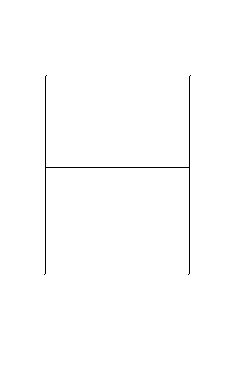
\includegraphics[width=.2\linewidth]{images/h-skel-inv}};
		\node[draw](k1) at (4,-3.5) {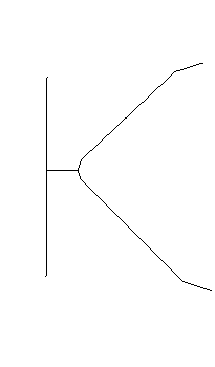
\includegraphics[width=.2\linewidth]{images/k-skel-inv}};
		\node[draw, label=below:{Skeletons}](z1) at (4,-7) {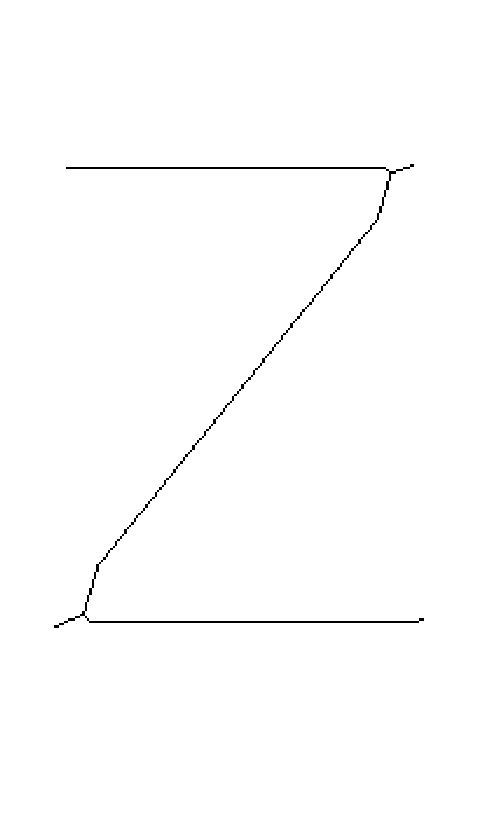
\includegraphics[width=.2\linewidth]{images/z-skel-inv}};
		
		\node[draw, circle, color=black, fill=white] (north) at (7,0) {};
		\node[draw, circle, color=black, fill=node] (n0) at (8,-2) {};
		\node[draw, circle, color=black, fill=node] (n1) at (8,-4) {};
		\node[draw, circle, color=black, fill=node] (n2) at (8,-6) {};
		\node[draw, circle, color=black, fill=node] (n3) at (10,-2) {};
		\node[draw, circle, color=black, fill=node] (n4) at (10,-4) {};
		\node[draw, circle, color=black, fill=node] (n5) at (10,-6) {};
		
		\draw[-, ultra thick] (north) to node [midway, fill=white] {4} (n0);
		\draw[-, ultra thick] (n1) to node [midway, fill=white] {1} (n0);
		\draw[-, ultra thick] (n1) to node [midway, fill=white] {1} (n2);
		\draw[-, ultra thick] (n1) to node [midway, fill=white] {1} (n4);
		\draw[-, ultra thick] (n4) to node [midway, fill=white] {1} (n3);
		\draw[-, ultra thick] (n4) to node [midway, fill=white] {1} (n5);
		
		\draw[->, ultra thick] (h0.east) to (h1.west);
		\draw[->, ultra thick] (k0.east) to (k1.west);
		\draw[->, ultra thick] (z0.east) to (z1.west);
		
		\draw[->, ultra thick] (h1.east) to ($(h1.east) + (1.5,-1)$);
		\draw[->, ultra thick] (k1.east) to ($(k1.east) + (1.5,0)$);
		\draw[->, ultra thick] (z1.east) to ($(z1.east) + (1.5,1)$);
		
		\node at (9,-7) {Output Graph};
	\end{tikzpicture}
	}
	
	\vspace{0.5em}
	
	\caption{Characters with isomorphic structure, which are thus ``identical'' \texttt{GlyphGraph} models.\label{fig:badisomorphism}}
\end{figure}

%\paragraph{An algorithm using path direction}
\subsection{A ``dual'' representation with path direction}
%?? introduce the ``dual'' representation (frame it like ``the graph models allowed me to learn \emph{why} these characters weren't distinct, and modify the algorithm to include path angle dynamics'')
In the framework established, it is difficult to capture the relationship between paths since they are modelled by edges.
To rework the model and enable these relationships to be captured, I start with a \emph{dual graph}-like conversion: edges in the prior model are converted into identically labelled vertices, placing an edge between these new vertices for each time their corresponding prior edges meet at the same vertex.
While this decision appears sensible since these labels \emph{are} the features recognised, to measure (and record) relative path angles it is insufficient to consider this transformation alone---\cref{alg:glyphgraph} measures and uses the start and end direction of each path segment, but these are not output.
A modification of the initial algorithm is thus required.

First we must divide our labellings into two classes: \emph{standard} features (lines and paths) which have well-defined directions at either end, and \emph{special} features (neighbourhood, north) which do not.
In the dual representation, edges between special$\leftrightarrow$regular edges are simply labelled `8' and special$\leftrightarrow$special edges are labelled `0'; the directional information becomes useful when considering regular$\leftrightarrow$regular relationships.
These directions are an integer in the range 0--7, numbering the neighbourhood pixels around a path's endpoint clockwise from north, and are assigned based on the location of the first point adjacent to that endpoint.
If two paths meet at a vertex, having directions $d$ and $d'$ at that point respectively, then their relationship is labelled $|d-d'|$.
Quite usefully, we \emph{can} return to the initial class of model from this new representation: each dual-vertex is transformed to an edge between two unknown vertices, which may be gradually inferred by iterating over the set of edges in the dual graph.

%?? changes core model -- MCS is now effectively ``edge-maximising'' relative to our prior model.
Theoretically, this new approach should increase matching performance.
The MCS procedure as I have defined it maximises the order of the produced common subgraph, yet the features in my first model lie on the edges.
Running this procedure on a dual graph-like transformation gives similar results to the \emph{maximum common edge subgraph} of the regular model, matching in a way that puts more emphasis on the count of features between a pair of graphs.

%?? old model is recoverable from new.

%====================================================
\section{Modifications to k-Down}
\label{sec:k-down-mods}
%====================================================

%?? Why? Attributed multi-graphs
Having seen that both of the proposed models take the form of attributed multigraphs, \citeauthor{Between-MCS-SIP}'s $k\downarrow$ requires adaptation to accommodate graphs as I have defined them.
%?? Discuss/introduce $s$-adjacency (Already added $N^{=}_{s},N^{\succcurlyeq}_{s}$ to graph definitions section), and 3 levels of filtering (induced, edge-count-increasing, barely overlapping)
The first step in matching these graphs is to determine which sequence-aware neighbourhood (and thus adjacency operator) will be used to impose the constraints arising from edge labels.
Each corresponds to a different level of filtering:
\begin{itemize}
	\item the exact neighbourhood $N^{=}_{s,\mathcal{G}}$ is necessary in the \emph{induced} variant of MCS, so that a pair of pattern and target vertex pairs may only map to one another if they have identical edge sequences;
	
	\item the overlap neighbourhood $N^{\circ}_{s,\mathcal{G}}$ provides the bare-minimum level of filtering needed when considering the \emph{non-induced} variant of MCS, allowing a pair of pattern and target vertex pairs to map to one another if there is any overlap in the edge sequences;
	
	\item the sufficient neighbourhood $N^{\succcurlyeq}_{s,\mathcal{G}}$, which allows a pattern vertex pair to be mapped to a target vertex pair if every edge in the former can be mapped to an edge of equal value in the latter, offering an oddly asymmetrical mapping when used in MCS---I define this (in the context of SIP) as building an \emph{edge-count-increasing subgraph isomorphism}.
\end{itemize}

\Cref{alg:k-down-search} then defines the necessary modifications to $k\downarrow$ to compute the MCS in each case.
%?? Filtering at top of search---modify loop constraints, vertex label matching
At the top of search, the matching procedure must enforce that vertices of $\mathcal{P}$ can only be mapped to vertices of $\mathcal{T}$ with equal labels.
Additionally, any vertices featuring loops must meet the selected sequence-adjacency criterion (lines \ref{alg:k-down-search:top-start}--\ref{alg:k-down-search:top-end}).
%?? Per-node of search, look at $s$-neighbourhoods
Per node of constraint propagation, domains are pruned using the chosen sequence-aware neighbourhood---if $v$ is mapped to $v'$ and $v$ and $w$ are adjacent with edge sequence $s$ in $\mathcal{P}$, then $w$ may only be assigned to vertices in the $s$-neighbourhood of $v'$ (lines \ref{alg:k-down-search:node-start}--\ref{alg:k-down-search:node-end}).

%?? Keep standard filtering from supplemental graphs (adjacency matrix operates on at least 1-adjacency, exact matches are provided)
The rest of the algorithm is unaffected by these additions; by providing both multigraph and simple graph notions of neighbourhood and adjacency, the existing filtering provided by supplemental graphs is maintained.
%?? Could use path-based inference for new supplemental graphs, but probably way too much work for graphs of this order (i.e.\ very small)
Admittedly, further supplemental graphs could be added, filtering on commonly seen label patterns in paths; although with the relatively low-order graphs produced by the examined models such optimisations would be largely unnecessary for this study.

\begin{algorithm}[t]
	\DontPrintSemicolon
	\caption{Modifications for k$\downarrow$ \cite{Between-MCS-SIP} for attributed multigraphs, given (for a graph $\mathcal{G}$) a vertex labelling function $\ell_\mathcal{G}$, a chosen multigraph neighbourhood function $\mathcal{N}_{s,\mathcal{G}}$ and its associated adjacency operator ``$\sim_{s,\mathcal{G}}$''. \label{alg:k-down-search}}
	\tcp{
%		replacement for lines 5--9\\
		top-of-search filtering with sequences on loop constraints}
	\ForEach{$v \in \operatorname{V}(\mathcal{P})$}{
		$D_v \leftarrow \operatorname{V}(\mathcal{T})$\;
		\ForEach{$(P,T)\in L$}{
			$D_v \leftarrow \{ w \in D_v : v \sim_P v \Rightarrow w \sim_t w \land S_P(v) \lesspreceq{k} S_T(w) \}$
		}
	
		\BlankLine
		$s \leftarrow \operatorname{seq}_{\mathcal{P}}(v,v)$\;\label{alg:k-down-search:top-start}
%		$Valids \leftarrow \{\}$\;
%		\ForEach{$w \in \operatorname{V}(\mathcal{T})$}{
%			\If{$v \sim_{\mathcal{P}} v \Rightarrow w \sim_{s,\mathcal{T}} w \land l_\mathcal{P}(v) = l_\mathcal{T}(w)$}{
%				$Valids \leftarrow Loops \cup \{w\}$
%			}
%		}
		$D_v \leftarrow \{ w \in D_v : \ell_\mathcal{P}(v) = \ell_\mathcal{T}(w) \land v \sim_P v \Rightarrow w \sim_{s,\mathcal{T}} w \}$\;\label{alg:k-down-search:top-end}
		$D_v \leftarrow D_v \cup k$ distinct wildcard vertices\;
	}
	
	\BlankLine
	\BlankLine
	\tcp{
%		replacement for lines 35--40\\
	filtering with sequences during propagation}
	\ForEach{$D_w \in D\backslash\lbrace D_v\rbrace$}{
		$D_w \leftarrow D_w \backslash \lbrace v'\rbrace$\;
		\ForEach{$(P, T) \in L$}{
			\If{$v \sim_P w$}{
				$D_w \leftarrow D_w \cap (N_T(v') \cup wildcards )$
			}
		}
		\BlankLine
		$(P_0, T_0) \leftarrow L[0] $\;\label{alg:k-down-search:node-start}
		\If{$v \sim_{P_0} w$}{
			$s \leftarrow \operatorname{seq}_{P_0}(v,w)$\;
			$D_w \leftarrow D_w \cap (\mathcal{N}_{s,T_0}(v') \cup wildcards )$\;\label{alg:k-down-search:node-end}
		}
		\If{$D_w = \emptyset$}{\Return{\textbf{false}}}
	}
\end{algorithm}

%====================================================
\section{Empirical Evaluation \& Discussion}
\label{sec:evaluation}
%====================================================

?? Machine statistics, find the code here\footnote{\url{https://github.com/FelixMcFelix/sip-for-cv-paper}}, roll up a nice VM for review?

?? Heatmaps per font -- examine size? font v font? sans vs serif? Dual vs regular? How do the different filtering levels affect character distinctness? Use the word ``curiously'' to describe relation between more distinct chars and reduced classifier performance.

?? Matching effectiveness statistics with HWRT \cite{HwrtDatabase} (Discuss effects of pen thickness, filtering class, dual vs regular). kNN classifier ($k=5$ I think)

?? What else? Try it out on the george washington letters dataset for direct comparison with \cite{Graphs-Handwriting}? IF NOT DONE, PUT IN FUTURE WORK

%====================================================
\section{Related Work}
\label{sec:related}
%====================================================

?? Handwriting analysis w/ kNN \cite{Graphs-Handwriting}

%====================================================
\section{Further Applications}
\label{sec:applications}
%====================================================

?? Give example of graph of two circuit diagrams here

?? Examine graph order---too big? Can we run SIP on it? How are the results?

%====================================================
\section{Conclusions}
\label{sec:conclusion}
%====================================================

?? Draw conclusions here---sum up paper.

?? Future work? Approximate GED metrics? Investigation of path-based supplemental graphs?

?? MCS/GED bad fit? i.e. p,q,b,d have small GED since all that moves is the north relation.

%====================================================
\noindent
{\bf Acknowledgments.}
%====================================================
This is optional; it is a location for you to thank people ?? TODO

%====================================================
\section{References}
%====================================================
\printbibliography[heading=none]

% Fix weird underhang of last reference
\vspace{1em}

\end{document}